% CVPR 2024 Paper Template; see https://github.com/cvpr-org/author-kit

\documentclass[10pt,twocolumn,letterpaper]{article}

%%%%%%%%% PAPER TYPE  - PLEASE UPDATE FOR FINAL VERSION
\usepackage{cvpr}              % To produce the CAMERA-READY version
% \usepackage[review]{cvpr}      % To produce the REVIEW version
% \usepackage[pagenumbers]{cvpr} % To force page numbers, e.g. for an arXiv version
\usepackage{wrapfig}
\usepackage{multirow}
\usepackage{makecell}
\usepackage{bbding}
\usepackage{color}

\usepackage{xcolor}
% \usepackage[table ]{xcolor}


% Import additional packages in the preamble file, before hyperref

% It is strongly recommended to use hyperref, especially for the review version.
% hyperref with option pagebackref eases the reviewers' job.
% Please disable hyperref *only* if you encounter grave issues, 
% e.g. with the file validation for the camera-ready version.
%
% If you comment hyperref and then uncomment it, you should delete *.aux before re-running LaTeX.
% (Or just hit 'q' on the first LaTeX run, let it finish, and you should be clear).
\definecolor{cvprblue}{rgb}{0.21,0.49,0.74}
\usepackage[pagebackref,breaklinks,colorlinks,citecolor=cvprblue]{hyperref}

%%%%%%%%% PAPER ID  - PLEASE UPDATE
\def\paperID{3945} % *** Enter the Paper ID here
\def\confName{CVPR}
\def\confYear{2024}

%%%%%%%%% TITLE - PLEASE UPDATE
\title{A Unified Framework for Human-centric Point Cloud Video Understanding}

%%%%%%%%% AUTHORS - PLEASE UPDATE
% \author{
%     Yiteng Xu\textsuperscript{\rm 1},
%     Kecheng Ye\textsuperscript{\rm 1},
%     Xiao Han\textsuperscript{\rm 1},
%     Yiming Ren\textsuperscript{\rm 1},
%     Xinge Zhu\textsuperscript{\rm 2},
%     Yuexin Ma\textsuperscript{\rm 1,}\thanks{Corresponding author. This work was supported by NSFC (No.62206173), Shanghai Sailing Program (No.22YF1428700), MoE Key Laboratory of Intelligent Perception and Human-Machine Collaboration (ShanghaiTech University), Shanghai Frontiers Science Center of Human-centered Artificial Intelligence (ShangHAI), Shanghai Engineering Research Center of Intelligent Vision and Imaging.}\\
% % Institution1\\
% % Institution1 address\\
% % {\tt\small \{xuyt2023,mayuexin\}@shanghaitech.edu.cn}
% \affiliations{
%    $^{1}$ShanghaiTech University 
%    $^{2}$ The Chinese University of Hong Kong
%    \\
%    \{xuyt2023,mayuexin\}@shanghaitech.edu.cn
% % See more examples next
% }
% }

\author{\textbf{
Yiteng Xu\textsuperscript{\rm 1},
Kecheng Ye\textsuperscript{\rm 1},
Xiao Han\textsuperscript{\rm 1},
Yiming Ren\textsuperscript{\rm 1},
Xinge Zhu\textsuperscript{\rm 2},
Yuexin Ma$^{1,}$\thanks{Corresponding author. This work was supported by NSFC (No.62206173), Shanghai Sailing Program (No.22YF1428700), MoE Key Laboratory of Intelligent Perception and Human-Machine Collaboration (ShanghaiTech University), Shanghai Frontiers Science Center of Human-centered Artificial Intelligence (ShangHAI), Shanghai Engineering Research Center of Intelligent Vision and Imaging.}
}\\ 
$^{1}$ ShanghaiTech University
$^{2}$ The Chinese University of Hong Kong \\
% $^{3}$ Shanghai AI Laboratory 
% $^{4}$ The Chinese University of Hong Kong\\
{\tt\small \{xuyt2023,mayuexin\}@shanghaitech.edu.cn}}

\begin{document}
\maketitle
\begin{abstract}
Human-centric Point Cloud Video Understanding (PVU) is an emerging field focused on extracting and interpreting human-related features from sequences of human point clouds, further advancing downstream human-centric tasks and applications. Previous works usually focus on tackling one specific task and rely on huge labeled data, which has poor generalization capability. Considering that human has specific characteristics, including the structural semantics of human body and the dynamics of human motions, we propose a unified framework to make full use of the prior knowledge and explore the inherent features in the data itself for generalized human-centric point cloud video understanding. Extensive experiments demonstrate that our method achieves state-of-the-art performance on various human-related tasks, including action recognition and 3D pose estimation. \textbf{All datasets and code will be released soon.}


%Recently, human-centric point cloud video understanding has become an emerging research field. The key challenge of this task is to extract the geometric and motion representation of dynamic human point clouds. Previous works use transformers to model the relationships among the features of flattened local spatial temporal tubes. However, these methods suffer from problems of high time expenditure and large memory consumption. Besides, these methods cannot track the motion of local fine-grained structures in the long term, which is essential in capturing the human motion feature more precisely. To solve this problem, we utilize prior geometric knowledge of the human body to deconstruct the human into body parts, then decouple the appearance and motion feature extraction by applying spatial modeling and temporal modeling respectively, which is more effective and efficient. Besides, inspired by the pre-trained LLM and LVM~\cite{devlin2018bert,radford2018improving,kirillov2023segment}, which apply self-supervised pre-training on large amounts of unlabeled data and perform well when fine-tuning on multiple downstream tasks, we build a pre-trained paradigm in human point cloud video using geometric and dynamic representation learning methods. Extensive experiments on several downstream tasks demonstrate the effectiveness of our proposed method.

% Recently, human-centric point cloud video understanding has become an emerging research field, which plays an indispensable role in real-world human-related applications. 
% The key challenge of this task is to extract the geometric and motion representation of dynamic human point clouds.
% Previous works use point tubes to extract the local spatial-temporal first, then model the global relationships among the tubes feature in long term videos using transformers.
% However, these methods suffer from problems of high time expenditure and large memory consumption.
% Besides, these methods are unable to build the one-to-one temporal correspondence of point tubes before and after, thus cannot track the local structure in the long term and extract the motion features of fine-grained structure in global context, which is of vital importance in capturing the human motion feature in point cloud videos.
% To solve this problem, we utilize prior knowledge of the human body to deconstruct the human into fine-grained parts, then decouple the geometric and motion feature extraction by applying spatial modeling and temporal modeling respectively, which is more effective and efficient. 
% Besides, Inspired by the pre-trained large language model and large vision model~\cite{devlin2018bert,radford2018improving,kirillov2023segment}, which apply self-supervised pre-training on large amounts of unlabeled data and performs well when fine-tuning on multiple downstream tasks, we build a pre-trained model in human point cloud video.
% Besides, Inspired by the pre-trained LLM and LVM~\cite{devlin2018bert,radford2018improving,kirillov2023segment}, which apply self-supervised pre-training on large amounts of unlabeled data and perform well when fine-tuning on multiple downstream tasks, we build a pre-trained model in human point cloud video using geometric and dynamic representation learning methods.
% Extensive experiments on HuCenLife~\cite{xu2023human}, LIP~\cite{ren2023lidar}, SUSTeck 1k~\cite{shen2023lidargait} demonstrate the effectiveness of our proposed method.




% Representation learning in point cloud has demonstrated promising development in recent years. Existing works mainly focus on the whole scene or objects, rather than humans whose spatial-temporal structure is more complicated and challenging.
% Recently, human-centric point cloud video understanding has become an increasingly popular research field, which plays an indispensable role in real-world human-related applications. To understand human motion better in multiple downstream tasks, we propose the Human-centric LiDAR 4D spatial-temporal multi-task unified framework.
% We utilize prior knowledge of the human body to deconstruct the human into fine-grained parts, then decouple the geometric and motion feature extraction by applying spatial modeling and temporal modeling on parts features respectively, which is more effective and efficient. We also use self-supervised learning methods to provide pre-trained network weights, which can perceive the essential spatial-temporal feature of human motion therefore can benefit multiple downstream tasks.
% Extensive experiments on HuCenLife~\cite{xu2023human}, LIP~\cite{ren2023lidar}, SUSTeck 1k~\cite{shen2023lidargait} demonstrate the effectiveness of our proposed method.

\end{abstract}    
\section{Introduction}
\label{sec:intro}

Human-centric point cloud video understanding (PVU) is a burgeoning field focused on discerning, interpreting, and quantifying human-related information within sequences of human point clouds. This area has witnessed a surge in attention in recent years, particularly applied in LiDAR captured large-scale unconstrained scenarios~\cite{xu2023human,dai2023sloper4d,yan2023cimi4d,han2022licamgait}. Its significance lies in its critical role in facilitating various downstream tasks, including human action recognition~\cite{xu2023human}, 3D pose estimation~\cite{cong2023weakly}, motion capture~\cite{ren2023lidar,li2022lidarcap}, etc. These advancements hold the potential to further drive progress in real-world applications, such as intelligent surveillance, assistive robots, human-robot collaboration, etc.


Current methods~\cite{xu2023human,ren2023lidar,li2022lidarcap} usually rely on extensive labeled data for supervision and employ generic point cloud-based feature extraction backbones~\cite{qi2017pointnet,qi2017pointnet++,ma2022rethinking,guo2021pct}. Nevertheless, obtaining the necessary data and annotations for 4D human-centric point cloud videos proves to be a challenging and expensive endeavor. Furthermore, fully supervised techniques tend to exhibit overfitting issues when applied to specific datasets or tasks, resulting in limited generalization capabilities. Additionally, the existing feature extraction networks are ill-suited for human-centric data, as they fail to account for human-specific characteristics. Hence, within the domain of human-centric PVU, the significance of self-supervised learning becomes evident in enhancing algorithmic generalization. Simultaneously, the development of a human-specific feature extractor that uses prior human-related knowledge holds great promise in bolstering the effectiveness of methods for downstream tasks.
\begin{figure}[t]
    \centering  
    \includegraphics[width=0.5\textwidth]
    {pic/teaser_point_level.drawio.pdf} 
    \caption{UniPVU-Human extracts human-related prior knowledge at global level, part level, and point level to facilitate subsequent geometric and dynamic representation learning, finally cater to a range of downstream human-centric tasks, such as action recognition, 3D pose estimation, etc.}
    \label{fig:overview}
 \end{figure}

Actually, self-supervised learning~\cite{wang2021self,zhang2023complete} for PVU has made great progress. Some approaches~\cite{sheng2023contrastive,sheng2023point,shen2023pointcmp} leverage contrastive learning techniques to capture essential spatio-temporal features within dynamic point clouds. Nevertheless, due to the inherent challenges posed by irregular point distributions stemming from varying capture distances, occlusions, and noise, the construction of high-quality positive and negative samples remains a nontrivial task, thereby making the optimization process difficult. The latest work~\cite{shen2023masked} exploits mask prediction for point cloud video self-learning by dividing sequential point clouds into tubes for masking and recovering. However, this method flattens all tubes for feature learning, inadvertently compromising the semantic and dynamic consistency in 4D videos. Moreover, all these methods are not tailored specifically to address human-centric PVU.


Given the importance of human-centric tasks, the imperative need arises to establish a unified framework for the understanding of human point cloud videos. Notably, no specific solutions to this challenge have been identified to date. In this paper, we approach the problem by addressing two fundamental questions: \textit{first, what human-related prior knowledge can be extracted, and second, how can the knowledge be harnessed to enhance human-centric representation learning}?

Considering the inherent structure of the human body, characterized by fixed components such as torso, head, arms, and legs, as well as the distinctive dynamic traits exhibited during human motion, we exploit both \textbf{the structural semantics of human body and human motion dynamics} to facilitate the acquisition of human-specific features from sequences of point clouds. In particular, we create two large-scale point-cloud-based datasets and corresponding pre-trained networks for body segmentation and motion flow estimation, respectively, so that human prior knowledge can be learned in advance and assist subsequent representation learning. 
Furthermore, within our framework, we introduce two innovative stages tailored to maximize the utility of this prior knowledge. The first one, termed \textbf{semantic-guided spatio-temporal representation self-learning}, incorporates a body-part-based mask prediction mechanism designed to facilitate the acquisition of geometric and dynamic representations of humans in the absence of annotations. Building upon this foundation, the following stage, \textbf{hierarchical feature enhanced fine-tuning}, integrates and adapts global-level, part-level, and point-level point cloud features to cater to a range of downstream tasks. In this way, our approach, named \textbf{UniPVU-Human}, serves as a comprehensive exploration of human prior knowledge, furnishing a unified framework for the effective learning of human-centric representations.


To evaluate the effectiveness of our method, we conduct extensive experiments on two popular LiDAR-point-cloud-based datasets~\cite{xu2023human,ren2023lidar}, focusing on human action recognition and human pose estimation, respectively. Our method achieves state-of-the-art performance on both tasks. Detailed ablation studies are also provided to verify each stage and technical design in our framework.

To summarize, our contributions are as follows:
\begin{enumerate}
    \item We propose UniPVU-Human, the first unified framework for human-centric point cloud video understanding, which is significant for vast downstream applications.
    \item Containing two novel stages, including semantic-guided spatio-temporal representation self-learning and hierarchical feature enhanced fine-tuning, our method fully takes advantage of prior knowledge of humans for effective and robust human-centric representation learning.
    \item Our method achieves state-of-the-art performance on open datasets for various human-centric tasks.
    
\end{enumerate}

%Modern intelligent robotics or autonomous vehicle are usually equipped with depth sensors like LiDAR or depth cameras, which can perceive the our dynamically changing 3D world by processing the point cloud sequences in various visibility environments. And human-centric point cloud video understanding becomes an emerging research field, for it plays an indispensable role in real-world human-related applications like autonomous vehicles, human-robot interaction and VR/AR. However, point cloud sequences are irregular and unordered spatially and inconsistent temporally, making it difficult to model the spatial-temporal structure in long term. Moreover, human body is non-rigid object which exists not only global rotations and translations but also local rotations and translations, such as relative movements among joints, which means it is more complicated and challenging to model the motion feature of human point cloud.

%Recent works~\cite{fan2021point,fan2022point,shen2023masked} select anchor frames to divide long point cloud video sequences in to clips containing several frames. Then they select spatial anchor points in anchor frames to build point tubes with nearest points around spatially and temporally, and apply 4D convolution to capture the local features. After that, they flatten the point tubes features within clips spatially and among clips temporally, and use Transformer among all tubes features to learn the global appearance and motion representation jointly. However, it suffers high time expenditure and large memory, for the consumption for the square time complexity of self-attention on flattened point tubes
%Besides, these methods don't build the one-to-one temporal correspondence of point tubes in adjacent clips. They flatten the tubes spatially and temporally and mix all tubes together, which destroy the original spatial geometric structure of human body in every frame and motion features of local fine-grained structure in long term, which is essential in capturing the relative movements among joints for non-rigid human body. 


%To address this problem, we utilize prior geometry knowledge of human body to deconstruct the human into fine-grained parts by a part segmentation network pre-trained on synthetic dataset., making it possible to decouple the appearance and motion feature extraction by applying spatial modeling and temporal modeling respectively, which is more effective and efficient. 

%Besides, most of 3D data entails labor-intensive human annotations~\cite{chen2023pointgpt}, which is expensive and time-consuming, causing the scale of existing 3D datasets much smaller than that of that of 2D datasets. Inspired by pre-trained Large Language Model(LLM) and Large Vision Model(LVM), ~\cite{devlin2018bert,radford2018improving,kirillov2023segment}, which apply self-supervised pre-training on large amounts of unlabeled data and performs well when fine-tuning on multiple downstream tasks, we fuse several LiDAR Human dataset into a million level large datasets and build a self-supervised pre-trained model using geometric and dynamic representation learning methods on it.
%Extensive experiments on HuCenLife~\cite{xu2023human}, LIP~\cite{ren2023lidar} demonstrate the effectiveness of our proposed method.

%To summarize, our contributions are as follows:
% The research in LiDAR-based human-centric video understanding ~\cite{li2022lidarcap,xu2023human,cong2023weakly,shen2023lidargait,ren2023lidar} has experienced rapid progress. 
% LiDAR can provide precise depth in large-scale scenarios, regardless of light or weather conditions, making it popular in many human-related applications like autonomous vehicles, human-robot interaction and VR/AR.
% A lot of new feature extractor has emerged, which performs well in specific tasks, such as action recognition~\cite{xu2023human}, 3D pose estimation~\cite{ren2023lidar,li2022lidarcap} or gait recognition~\cite{ren2023lidar}. 
% The key challenge of these tasks is to extract the geometric and motion representation of dynamic human point clouds. However, point cloud sequences are irregular and unordered spatially and inconsistent temporally, making it difficult to model the spatial-temporal structure of human motions. Besides, point clouds are semantically sparse but redundant in consecutive frames, therefore the balance between


% Some works apply self-supervised representation learning methods on point cloud video understanding ~\cite{sheng2023contrastive,shen2023pointcmp,shen2023masked,sheng2023point}. They divide the video into small clips first, and then extract spatial-temporal features from each clip independently. Afterwards, they explore the long term temporal relationship among clip features.
% However, these methods model temporal relationships at global frame scale, ignoring the long term motion of fine-grained local structure of point cloud, for it's challenging to track local structures in consecutive point cloud frames.
% As a result, motion features extracted from these methods are coarse and redundant.


% Nevertheless, The human body has special geometric characteristics, for a person is composed of fixed body parts. Therefore, we use part segmentation to partition the human body in this paper. Through tracking the body part in a long term, we can model the motion representation of humans more precisely. 
% Besides, we also extract features of all parts in every single frame to capture global geometric representation.
% Last but not least, We fuse human motion flow with points in fine-tuning stage, enhancing the model's ability to extract geometric and motion features in multiple levels, i.e. global instance level, body part level, and point-wise level simultaneously.


% Compared to contrastive learning based methods~\cite{sheng2023point,xue2023ulip}, mask reconstruction based self-supervised pre-training methods~\cite{pang2022masked,zhang2022point} perform better in capturing fine-grained local features, which has been widely applied in static point cloud representation learning but less explored for point cloud videos. 
% We set body part embedding as attention token and design a spatial-temporal mask-reconstruction module in pre-training stage, including a spatial-temporal transformer encoder, a decoder and a reconstruction head.
% We randomly mask some part patches in temporal and spatial dimension of point cloud video as well as a proportion of points in visible part left, encouraging the encoder networks to  extract high-level latent geometric and motion feature of human from incomplete point clouds through reconstructing the mask point clouds.


% Since our model learns from data itself without manually annotated supervision information, the representations learned by our model are not task-specific but the essential local and global human geometry and motion features.
% Therefore, it can be transferred to various downstream tasks, making it a multi-task unified framework.
% During fine-tuning, we discard the decoder and add task-specific heads, and achieve state-of-the-art performance in action recognition, 3D pose estimation, and gait recognition.

% To summarize, our contributions are as follows:

% •	We partition the point cloud of human into several body parts, establishing the long-term correspondences of each part in long point cloud sequences. Through spatial and temporal modeling of body parts, our model can capture geometric and motion feature of fine-grained local structure more precisely.

% •	We design a self-supervised spatial-temporal mask reconstruction module, enabling the encoder network to learn high-level spatial-temporal latent representations in pre-training stage, which can be finetuned on various downstream tasks, leading to a multi-task unified framework in human-centric LiDAR point cloud video understanding.

% •	We add human motion flow to LiDAR points, enhancing the model's ability to extract motion features in global instance level, body part level, and point-wise level simultaneously.



\section{Related Work}
\label{sec:related_work}
\begin{figure*}[t]
    \centering
    \includegraphics[width=2.1\columnwidth]{pic/main_figure_with_graph_new_token.drawio.pdf}
    \caption{The main pipeline of UniPVU-Human, which can be divided into three stages, including (a) Prior Knowledge Extraction, (b) Semantic-Guided Spatio-temporal Representation Self-learning, and (c) Hierarchical Feature Enhanced Fine-tuning. First, the pre-trained HBSeg and HMFlow are used to provide geometric and dynamic information, including body part segmentation results and point-wise motion flow. Then, our self-learning stage incorporates a body-part-based mask prediction mechanism designed to facilitate the acquisition of geometric and dynamic representations of humans in the absence of annotations. Finally, we integrate global-level, part-level, and point-level features to boost the knowledge transfer to downstream tasks in the fine-tuning stage. } 
    \label{fig:main_figure}
    \vspace{-1ex}
\end{figure*}
\subsection{Feature Learning for Point Clouds}
Point cloud is an important representation for 3D scenes and objects, and tremendous efforts have been made~\cite{ma2022rethinking,qian2022pointnext} for extracting valuable features from point clouds. PointNet~\cite{qi2017pointnet} is to learn a spatial encoding of each point and then aggregate all individual point features to a global point cloud signature\cite{qi2017pointnet++}.
PointNet++\cite{qi2017pointnet++} further introduces a hierarchical feature learning paradigm to capture the local geometric structures recursively. 
PointNeXt~\cite{qian2022pointnext} revisits PointNet++\cite{qi2017pointnet++} with improved
training and scaling strategies.
PCT~\cite{guo2021pct} and PointTransformer~\cite{zhao2021point} apply attention-based mechanism~\cite{vaswani2017attention} to point cloud representations.
Subsequently, many methods~\cite{choy20194d,liu2019meteornet,choy20194d,fan2022pstnet} extend them to process dynamic point cloud videos for more extensive applications.  
%MinkowskiNet~\cite{choy20194d} uses 4D sparse convolution on 4D occupancy grid converted from point clouds and PSTNet~\cite{fan2022pstnet} constructs the spatio-temporal convolution hierarchically.
%3DV~\cite{wang20203dv} employs a temporal rank pooling to integrate point motion into a voxel set and then extracts the spatio-temporal representation using PointNet++.
%MeteorNet~\cite{liu2019meteornet} appends a temporal dimension to PointNet++ to process 4D point clouds.
P4Transformer~\cite{fan2021point} and PST-Transformer~\cite{fan2022point} use transformers among all local 4D tubes' features to capture long relationships. With the development of autonomous driving, some works~\cite{voxelnet,zhu2021cylindrical,centerformer,centerpoint} propose voxel-based or voxel-point-based feature extractors to process LiDAR point clouds for high efficiency.
However, all these methods are not specifically designed for human dynamic point clouds, lacking the consideration of human-specific characteristics. 

\subsection{LiDAR-based Human-centric Understanding}
Recently, the understanding of human-centric point cloud videos, which are captured by LiDARs in large-scale scenes, has become an emerging field with a lot of new datasets and benchmarks for various human-centric tasks. 
LiDARCap~\cite{li2022lidarcap} contributes an in-the-wild human motion dataset and proposes a LiDAR point cloud video-based motion capture framework. Subsequent works, LIP~\cite{ren2023lidar}, explores the feature fusion of different visual sensors to address 3D pose estimation task based on point clouds and images. 
% Some works~\cite{shen2023lidargait,han2022licamgait} leverage point cloud videos to recognize the human gaits with the help of 3D geometric information. 
Recently, HuCenLife~\cite{xu2023human} proposes a huge human-centric dataset with diverse daily-life scenarios and rich human activities, and provides baselines for human perception, action recognition, motion prediction, etc. However, all these approaches follow previous generic backbones to extract features from sequence human point clouds without making use of human prior knowledge. Moreover, they are all supervised methods, causing unsatisfactory results when generalizing to other datasets or tasks.


\subsection{Self-supervised Learning for Point Clouds}
To understand the point cloud representation from data itself instead of supervision by manual annotations, some methods improve the generalization capability via self-learning in the pre-training stage. There exist many methods~\cite{xie2020pointcontrast,yu2022point,pang2022masked,zhang2022point,chen2023pointgpt} learning the geometric representation from static point cloud in a self-supervised manner. Recently, more and more self-learning methods~\cite{wang2021self,zhang2023complete} are proposed to learn the spatio-temporal representations of point cloud videos. Some approaches~\cite{sheng2023contrastive,sheng2023point,shen2023pointcmp} adopt contrastive learning spatially and among frames to learn inherent geometric and dynamic features. However, LiDAR point clouds are sparsity-varying across different capture distances, are usually incomplete due to occlusions, and contain undesired noises, making these methods unstable due to low-quality positive and negative pairs. In the recent study~\cite{shen2023masked}, mask prediction~\cite{he2022masked} is employed for self-learning in point cloud videos by segmenting sequential point clouds into tubes. However, it flattens all tubes during feature learning, inadvertently affecting the semantic and dynamic consistency in 4D videos. Additionally, all these methods lack customization for the specific requirements of human-centric point cloud video understanding.


%PointContrast~\cite{xie2020pointcontrast} used contrastive loss to associated matched point pairs in two views of point cloud generated from various data augmentations. PointBERT~\cite{yu2022point} introduced masked point modeling to predict the latent representation from an offline tokenizer. PointMAE~\cite{pang2022masked} solved the problem of position information leakage of PointBERT by shifting the mask tokens to the decoder and only input unmasked tokens into encoder. PointM2AE~\cite{zhang2022point} additionally utilizes a hierarchical transformer architecture of PointMAE to extract the multi scale representation of point clouds.PointGPT~\cite{chen2023pointgpt} arranges point patches in an ordered sequence exploit the GPT scheme for point cloud self-supervised learning.

%Recently, self-supervised learning methods are proposed to learn the spatial-temporal representation of point cloud video or sequences better. 
%Wang et al.~\cite{wang2021self} designs pretext task to pre-train dynamic point cloud networks by predicting the temporal order of shuffled segments.
%C2P~\cite{zhang2023complete} input the complete and partial sequences to teacher and student networks respectively and develop complete-to-partial 4D knowledge distillation. 


%(Remaining Contrastive Predictive Autoencoders for Dynamic Point Cloud~\cite{sheng2023contrastive}, 

%PointCMP Contrastive Mask Prediction for Self-supervised Learning~\cite{shen2023pointcmp}, 

%Point Contrastive Prediction with Semantic Clustering for Self-Supervised Learning on Point Cloud Videos~\cite{sheng2023point}, 

%Masked Spatio-Temporal Structure Prediction for Self-supervised Learning~\cite{shen2023masked})





% \subsection{Self-supervised Representation Learning in Indoor Point Cloud Video }
% \subsection{Indoor Point Cloud Video Understanding Based on Depth Cameras}
% For some indoor datasets like~\cite{shahroudy2016ntu,li2010action} based on depth or RGB-D cameras, a few works~\cite{liu2019meteornet,wen2022point,zhong2022no,fan2022pstnet,fan2021point,fan2022point,sheng2023contrastive,shen2023pointcmp,shen2023masked,sheng2023point} attempt to build dynamic models to process point cloud videos.
% ~\cite{fan2022pstnet,fan2021point,fan2022point} select anchor frames to divide long point cloud video sequences in to clips containing several frames. Then they select spatial anchor points in anchor frames to build point tubes and apply 4D convolution to capture the local spatial-temporal features. After that, PSTNet ~\cite{fan2022pstnet} continues to apply 4D convolution on point tubes to form a stacked convolutions, which limits the temporal modeling range by observing only a few frames~\cite{fan2022point}. P4Transformer~\cite{fan2021point} and PST-Transformer~\cite{fan2022point} use transformer to build the global relationships among all tubes features.
% Based on these methods, ~\cite{sheng2023contrastive,shen2023pointcmp,sheng2023point,shen2023masked} employ self-supervised pre-training by contrastive learning or mask prediction to learn appearance and dynamic representation of point cloud videos. 

% However, applying transformer on all point tubes to model global spatial-temporal representation jointly suffers high time expenditure and large memory consumption for the square time complexity of self-attention on flattened point tubes($O(T*N)^2$, where $T$ is the number of clips and $N$ is the number of tubes in a clip). 
% Besides, these methods don't build the one-to-one temporal correspondence of point tubes in adjacent clips, thus cannot track the local structure in long term to extract the motion features of fine-grained structure in global context, which is of vital importance in capturing the geometric and motion feature of human point clouds. In our method, we utilize prior knowledge of human body to deconstruct the human into fine-grained parts, then decouple the geometric and motion feature extraction by applying spatial modeling and temporal modeling respectively, which is more effective and efficient.
% \subsection{Human-centric Outdoor Point Cloud Video Understanding Benchmarks Based on LiDAR}
% Recently, the perception and understanding on LiDAR-based human-centric point cloud video sequence has become an emerging field with a lot of new datasets and benchmarks~\cite{li2022lidarcap,xu2023human,cong2023weakly,shen2023lidargait,ren2023lidar}. LiDARCap~\cite{li2022lidarcap} contributes a human motion capture dataset at a long range. 
% Then some methods like LIP~\cite{ren2023lidar} and FusionPose~\cite{cong2023weakly} explore the feature fusion of different visual sensors to perform pose estimation task with multimodal datasets. 
% LiDAR is also used to recognize the human gait~\cite{shen2023lidargait} and outperforms 2D methods by leveraging the 3D geometric information. HuCenLife~\cite{xu2023human} is the first LiDAR dataset collected in real daily-life scenarios with rich human activities. 
% However, most of these works design task-specific methods on corresponding benchmark, hence there does not exist a multi-tasks unified framework for human-centric LiDAR-based point cloud video understanding. In this work, we propose such framework by making full use of the geometric and motion feature of LiDAR human.

% \subsection{ Scene Flow in Point Cloud}
% \label{subsec:scene_flow}
% Scene flow estimation is a fundamental task that estimates the dense 3D displacement vectors of points from two consecutive frames~\cite{cheng2023multi}.
% In recent years, there has been rapid progress in scene flow estimation in point cloud~\cite{cheng2023multi,huang2022dynamic,ding2022fh,puy2020flot,liu2019flownet3d,wang2023ihnet,teed2021raft,lang2023scoop,shen2023self}. FlowNet3D~\cite{liu2019flownet3d} designs a flow embedding layer which mix the feature of two consecutive point cloud frames extracted from PointNet++~\cite{qi2017pointnet++}. FLOT~\cite{puy2020flot} casts the task of scene flow estimation as finding soft correspondences on a pair of point clouds via solving an optimal transport problem~\cite{li2023deep}. RAFT-3D~\cite{teed2021raft} estimates the dense flow field by iteratively updating the SE3 field with the constructed 4D correlation volume~\cite{dong2023nsm4d}.

% Based on these scene flow estimators, some methods build models to extract the motion feature of dynamic point clouds. MeteorNet~\cite{liu2019meteornet} use scene flow estimator to construct point-wise spatiotemporal neighborhoods. NSM4D~\cite{dong2023nsm4d} estimate scene flows by pretrained RAFT-3D~\cite{teed2021raft} to update the motion features of point cloud videos. However, most of these works focuses on rigid transformations in scenes. For non-rigid objects like the human body, there exist not only global rotations and translations but also local rotations and translations, such as relative motions among joints, which is more complicated and challenging. To address this problem, we create a synthetic dataset with human motion flow ground truth to train the flow estimator, which can provide point-wise motion information to benefit the motion feature extraction of point cloud humans.
\label{sec:method}

\section{Method}
The whole architecture of our method is presented in Figure.~\ref{fig:main_figure}. A point cloud video sequence for human instances is denoted as $PC \in 
 \mathcal{R}^{L \times N \times D}$, where $L$ is the sequence length, $N$ is number of points in each frame, and $D$ is the dimension of each point. 
To exploit both the structural semantics of human body and human motion to facilitate the acquisition of human-specific features from sequences of point clouds, we create two large-scale point-cloud-based datasets and corresponding pre-trained networks for body segmentation and motion flow estimation in \textbf{Prior Knowledge Extraction}.
% so that human prior knowledge can be learned in advance and assist subsequent representation learning. 
Besides, to learn the essential geometric and dynamic representations of humans from data itself, we explore the spatial and temporal relationships of structural semantics in human body by applying spatio-temporal modeling upon the embedding of body parts in the stage of \textbf{Semantic-guided Spatio-temporal Representation Self-learning}.
%compared to recent work~\cite{shen2023masked} who establish global relationships among flattened tubes built from FPS sampling and clustering which inadvertently compromises the semantic and dynamic consistency in 4D videos. 
Building upon this foundation, we use extracted multiple levels of human-related prior knowledge to benefit various downstream tasks by \textbf{Hierarchical Feature Enhanced Fine-tuning}, which integrates global-level, part-level, and point-level point cloud features.



\subsection{Prior Knowledge Extraction}
Different from the movements of rigid objects such as vehicles in traffic scenarios, the motion of non-rigid humans is more complicated, for it contains not only global rotations and translations but also local rotations and translations, such as relative motions among joints, making capturing human motion features more challenging. The key to addressing this problem is to model the human motion in more fine-grained levels, including body part level and point-wise level. Therefore, we build the Human Body Segmentation (HBSeg) and Human Motion Flow (HMFlow) networks to provide more fine-grained geometric and motion information about human body, which can serve as prior knowledge to facilitate following human-centric representation learning.
% Therefore, we pre-trained the HMFlow on synthetic data to provide point-wise motion information and benefit the enhancement of the hierarchical features when fine-tuning on downstream tasks.
\subsubsection{Human Body Segmentation (HBSeg)}
\begin{figure}[h]
    \centering  
    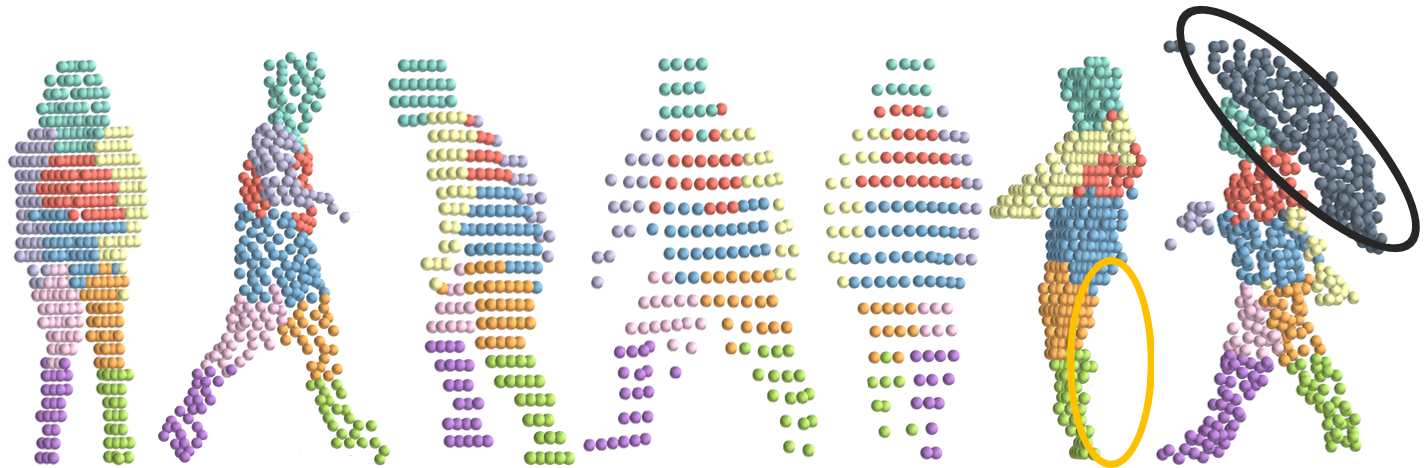
\includegraphics[width=0.5\textwidth]
    {pic/part_black_noise.png} 
    \caption{Visualization results of HBSeg on HuCenLife~\cite{xu2023human}.
    We show cases with different densities of LiDAR point cloud, occlusion (yellow circle), and noise (black circle). HBSeg has robust performance even merely trained on our synthesized dataset.}

    
    
    
    \label{fig:partseg_6.png}
 \end{figure}




\label{subsec:HBPSegModule}
To fully utilize the structural semantics of human body, we deconstruct human into fine-grained body parts by HBSeg, pre-trained on our synthetic dataset, which is constructed by employing a simulated LiDAR model~\cite{ren2023lidar} to scan the surfaces of 3D human meshes from the AMASS dataset~\cite{mahmood2019amass} at various perspectives and distances, meanwhile introducing random occlusions and noise to minimize the distribution gap between synthetic data and real data. We define 9 parts of human body and generate annotations by attaching the body part label of the nearest SMPL~\cite{loper2023smpl} mesh vertex to the synthetic LiDAR Point. More details are in Section.~\ref{subsubsec:HBPSegData} and supplementary material.

We adopt the PointNeXt-L~\cite{qian2022pointnext} as the main body network of HBSeg. 
After training on synthetic data, we apply the pre-trained HBSeg on real data to get the part segmentation labels $S \in \mathcal{R}^{L \times N \times 1}$. As Figure.~\ref{fig:partseg_6.png} shows, HBSeg performs stable on real-life data with changing sparsity and works well even for occlusion and noise cases, mainly due to our efforts on generating realistic synthetic data.
%For missing parts, we use information from adjacent frames to complete them.
% \begin{figure*}[t]
%     \centering
%     \includegraphics[width=2.2\columnwidth]{pic/part_seg.drawio.pdf}
%     \caption{Visualization of Human Body Part Segmentation(HBPSeg) geometric
%      }
%     \label{fig:vis_HBPSeg}
%     \vspace{-1ex}
% \end{figure*}


\subsubsection{Human Motion Flow Estimation (HMFlow)}



\begin{figure}[h]
    \centering  
    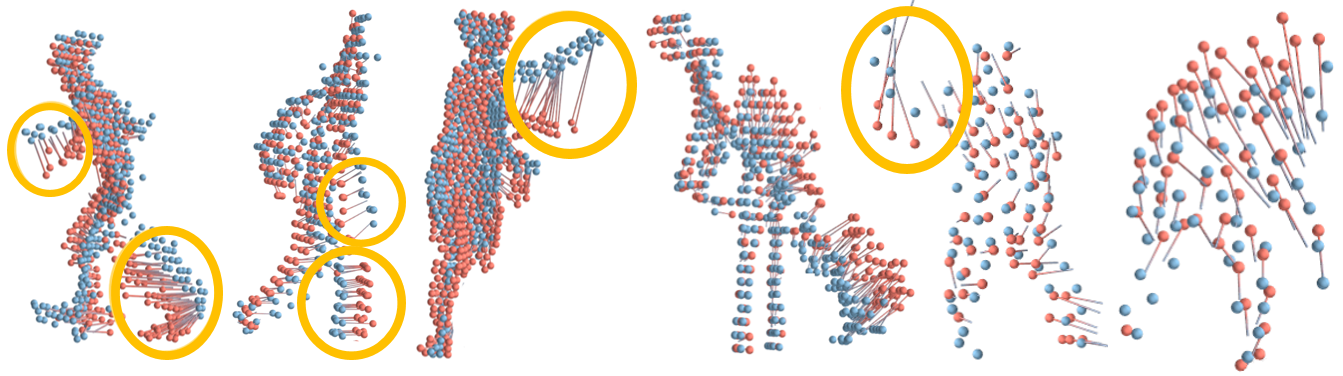
\includegraphics[width=0.46\textwidth]{pic/motion_sorted.png}  
    \caption{Visualization results of HMFlow on HuCenLife~\cite{xu2023human}. We present several cases from near to far relative to the LiDAR sensor. HMFlow has good capability of estimating point flow even for the parts with significant movements (yellow circle), which can provide explicit features of human dynamics.}


    % from dense to sparse. Yellow circles represent significant movements of human parts like waving arms and stretching legs. Our motion flow can track the movement, enabling us to better extract dynamic features.
    \label{fig:vis_HMFlow}
 \end{figure}


\label{subsec:HMFlowModule}
% However, most of these works focuses on rigid transformations in scenes. For non-rigid objects like the human body, there exist not only global rotations and translations but also local rotations and translations, such as relative motions among joints, which is more complicated and challenging. To address this problem, we create a synthetic dataset with human motion flow ground truth to train the flow estimator, which can provide point-wise motion information to benefit the motion feature extraction of point cloud humans.
% Different from the movements of rigid objects such as vehicles in traffic scenarios, the motion of non-rigid humans is more complicated, for it contains not only global rotations and translations but also local rotations and translations, such as relative motions among joints, which means capturing human motion features is more challenging. The key to address this problem is to model the human motion in more fine-grained levels, such as body part level or point-wise level. 
We pre-train the HMFlow on our synthetic dataset to provide point-wise motion information, which can benefit the feature enhancement in the fine-tuning stage.
Similar to Section.~\ref{subsec:HBPSegModule}, we associate each synthetic LiDAR point to its nearest SMPL vertex. Therefore, we are able to establish the correspondence between synthetic LiDAR points across different frames by using SMPL vertices indices, so that we can obtain motion flow ground truth for training our HMFlow. More details are in Section.~\ref{subsubsec:HMFlowData} and supplementary material.

We employ FLOT~\cite{puy2020flot} as the human motion flow estimator, which casts the task of scene flow estimation as finding soft correspondences on a pair of point clouds via solving an optimal transport problem~\cite{li2023deep}. When testing on the real data, we input adjacent LiDAR point clouds $PC_t$ and $PC_{t+1} \in \mathcal{R}^{L \times N \times D}$ into the pre-trained HMFlow to obtain human motion flow vectors $F \in \mathcal{R}^{L \times N \times D'}$ for each LiDAR point in the t-th frame. As Figure.~\ref{fig:vis_HMFlow} demonstrates, HMFlow can generate reasonable prediction for point-wise motion flow on real data even without annotations, which is valuable to provide explicit priors for human dynamics.

% The latent features of $F$ will be fused with those of points in our  in the fine-tuning stage, therefore we fully extract the information in point level which contains the point-wise position, motion direction and motion displacement. 
% Finally, we obtain three levels of representation for human-centric LiDAR point cloud videos: global human instance level, local body parts level, and point-wise level. Our model achieve good performance by making full use of information in three levels .


\subsection{Semantic-guided Spatio-temporal Representation Self-learning}
\label{subsec:STMaskRecon}
Due to spatial irregularities and temporal redundancies, annotating dynamic point cloud videos is labor-intensive and error-prone. Moreover, fully-supervised methods usually overfit to manual annotations in specific domains, struggling to capture the underlying patterns of new data~\cite{zeng2023self}. This limitation leads to a restricted ability to generalize to other tasks or datasets. Additionally, existing feature extraction networks employ generic point-cloud-based backbones that are ill-suited for human-centric data, as they do not account for human-specific characteristics.
Based on structure semantics of human bodies obtained in previous stage, we propose a module, named Semantic-guided Spatio-temporal Representation Self-learning, which mines essential geometric and motion features from human point cloud video data itself by masking and predicting body part patches to enhance the generalization ability of the model to benefit a variety of downstream tasks.

As Figure.~\ref{fig:main_figure} shows, We first mask some of the body-part tokens in temporal and spatial dimensions. After extracting the token embedding of part patches, only visible tokens will be input to the STEncoder to extract latent representation, which will be decoded with masked tokens together to reconstruct the 3D Cartesian coordinates of masked part patches. Details are as follows.




\subsubsection{Spatio-temporal Masking Strategy}
In temporal dimension, we mask all part patches in some random frames and reconstruct the masked tokens, encouraging STEncoder networks to estimate the part motion over a long period.
In spatial dimension, we randomly mask some part patches in the remaining frames after temporal masking, making the STEncoder network estimate the spatial geometric features of the entire human based on the visible tokens.

We apply temporal masking first, and then spatial masking. Given part patches $P \in \mathcal{R}^{L \times M \times N' \times D}$, we adopt a temporal mask ratio $r_t$ and spatial mask ratio $r_s$, respectively. Firstly, all part patches in $r_tL$ frames are masked, named as temporal masked patches $P_M^t \in \mathcal{R}^{r_tL \times M \times N' \times D}$, which will be used as the reconstruction ground truth of temporal masking. For every frame of the remaining $(1-r_t)L$ visible frames, $r_sM$ part patches are masked randomly, hence spatial masked patches $P_M^s \in \mathcal{R}^{(1-r_t)L \times r_sM \times N' \times D}$ will be used as the reconstruction ground truth of the spatial masking.

\subsubsection{Embedding Layer}
\label{subsubsec:embedding}
For visible part patches, we use Mini-PointNet~\cite{qi2017pointnet} as a tokenizer to obtain visible part tokens embedding $T_V$ from visible part patches $P_V$. 
\begin{equation}
    \begin{aligned}
    T_V = Tokenizer(P_V),
    \end{aligned}
\end{equation}
where $T_V \in \mathcal{R}^{(1-r_t)L \times (1-r_s)M \times C}$, $P_V \in \mathcal{R}^{(1-r_t)L \times (1-r_s)M \times N' \times D}$. $C$ is the channel dimension of part tokens. 
 % The features of motion flow will only be element-wise added to those of part tokens in fine-tuning stage to prevent the leakage of location information to the STEncoder in pre-trained stage.
For every masked part patch, we replace it with a share-weighted learnable masked part token $T_M$, which will be concatenated with the output of STEncoder and processed by the decoder together.

Learnable spatial positional encoding and temporal positional encoding will also be added to the input of every transformer layer in the STEncoder and decoder. 


\subsubsection{Spatio-temporal Encoder (STEncoder)}

To fully utilize the inherent structure of the human body, characterized by fixed components such as torso, head, arms, and legs, as well as the distinctive dynamic traits exhibited during human motion, our STEncoder applies spatial modeling and temporal modeling on body part tokens, respectively.
The STEncoder learns to extract the high-level latent geometric and motion features of humans from only $T_V$, which are input to STEncoder to get enhanced visible part tokens $T_V^E$.

For the network design of STEncoder, we interlace multiple spatial transformer~\cite{vaswani2017attention} layers and temporal transformer layers to extract the spatial geometry feature and temporal motion feature, respectively. For each spatial transformer layer, we apply self-attention~\cite{vaswani2017attention} among all visible parts tokens in every frame:
\begin{equation}
    \begin{aligned}
    V^{s'}_T = SpatialTransformer(V^{s}_T),
    \end{aligned}
\end{equation}
where $V^{s}_T, V^{s'}_T \in \mathcal{R}^{(1-r_s)M \times C}$ are the visible part tokens in a frame. For each temporal transformer layer, we apply self-attention for every visible part token among all L frames:
\begin{equation}
    \begin{aligned}
    V^{t'}_T = TemporalTransformer(V^{t}_T),
    \end{aligned}
\end{equation}
where $V^{t}_T, V^{t'}_T \in \mathcal{R}^{(1-r_t)L\times C}$ are the visible part tokens of a body part in $L$ frames.

\subsubsection{Mask Reconstruction}
Our decoder is similar to the STEncoder with fewer layers. We take the enhanced visible part tokens $T_V^E$ as well as masked part token $T_M$ as the input of the decoder. 
\begin{equation}
    \begin{aligned}
    T_R = Decoder(Concate(T_V^E,T_M)),
    \end{aligned}
\end{equation}
where $T_R \in \mathcal{R}^{L \times M \times C}$ is reconstructed part tokens.

Among the $T_R$, only the tokens masked before will be fed to the reconstruction head to predict the original masked part patches. The structure of the reconstruction head is similar to that in Point-MAE~\cite{pang2022masked}, which is a fully connected (FC) layer with a reshape operation.
\begin{equation}
    \begin{aligned}
    P^s_R = Reshape(FC(T^s_R)), \\
    P^t_R = Reshape(FC(T^t_R)), 
    \end{aligned}
\end{equation}
where $P^s_R \in \mathcal{R}^{(1-r_t)L \times r_sM \times N' \times D}$, $T^s_R \in \mathcal{R}^{(1-r_t)L \times r_sM \times C}$, $P^t_R \in \mathcal{R}^{r_tL \times M \times N' \times D}$, $T^t_R \in \mathcal{R}^{r_tL \times M \times C}$ are spatial reconstructed part patches, spatial reconstructed part tokens, temporal reconstructed part patches, temporal reconstructed part tokens, respectively.
We first reconstruct the spatial masked tokens, and then the temporal masked tokens. We adopt Chamfer Distance~\cite{fan2017point} Loss $L_{CD}$ as the reconstruction loss function:

\begin{equation}
    \begin{aligned}
    L_{CD} (P_M,P_R) = \frac{1}{\|P_M\|}\sum_{x \in P_M}\min_{y \in P_R}\|x-y\|_{2}^2 \\
    +\frac{1}{\|P_R\|}\sum_{y \in P_R}\min_{x \in P_M}\| y-x \|_{2}^2.
    \end{aligned}
\end{equation}
% where $MP_s \in \mathcal{R}^{(1-r_t)T \times r_sM}$ are Spatial Mask Patches served as the ground truth of spatial reconstruction.
% \begin{equation}
%     \begin{aligned}
%     L^t_{CD} (MP_t,RP_t) = \frac{1}{\|MP_t\|}\sum_{x \in MP_t}\min_{y \in RP_t}\|x-y\|_{2}^2 \\
%     +\frac{1}{\|RP_t\|}\sum_{y \in RP_t}\min_{x \in MP_t}\| y-x \|_{2}^2
%     \end{aligned}
% \end{equation}
% where $MP_t \in \mathcal{R}^{r_tT \times M}$ are Temporal Mask Patches served as the ground truth of temporal reconstruction.

\subsection{Hierarchical Feature Enhanced Fine-tuning}
\label{subsec:finetine}
After the above self-learning process, STEncoder is endowed with the ability to extract the representations of humans in part-level structural semantics. When fine-tuning on multiple downstream tasks, hierarchical features can enhance the STEncoder to capture more complicated and challenging fine-grained geometric and dynamic representations.
Specifically, we integrate global-level, part-level, and point-level point cloud features to pre-trained STEncoder (See Figure.~\ref{fig:main_figure}), therefore fully leveraging prior knowledge for effective and robust human-centric representation learning. 
 

During this stage, all part patches are visible to the STEncoder, and information of point-wise motion flow vector will be fused to that of body parts in Tokenizer. (See details in supplementary materials)
\begin{equation}
    \begin{aligned}
    T = Tokenizer(P,F),
    \end{aligned}
\end{equation}
where $T \in \mathcal{R}^{L \times M \times C}, P \in \mathcal{R}^{L \times M \times N' \times D}, F \in \mathcal{R}^{L \times M \times N' \times D'}$ are part tokens, part patches, and motion flow vectors, respectively. We will also append a global token extracted from the entire human instance to enable the interaction of features between global and part. For classification tasks like action recognition, a class token will be appended as well.
we discard the decoder and add corresponding task heads after the pre-trained tokenizer, learnable position encoding, and STEncoder for different tasks.

\section{Experiments}
\label{sec:experiments}
\begin{table*}\scriptsize 
\caption{Action Recognition in HuCenLife~\cite{xu2023human}.  $^{\dag}$ means adding global token and motion flow to these methods fair comparisons.}
\begin{tabular}{l|r|r|r|r|r|r|r|r|r|r|r|r|r}
\Xhline{1px}
                       & \multicolumn{1}{l|}{lift} & \multicolumn{1}{l|}{carry} & \multicolumn{1}{l|}{move} & \multicolumn{1}{l|}{pull\_push} & \multicolumn{1}{l|}{sco-bal} & \multicolumn{1}{l|}{hum-inter} & \multicolumn{1}{l|}{fitness} & \multicolumn{1}{l|}{entertain} & \multicolumn{1}{l|}{sports} & \multicolumn{1}{l|}{bend-over} & \multicolumn{1}{l|}{sit} & \multicolumn{1}{l|}{walk-stand} & \multicolumn{1}{l}{mAcc} \\ \hline
PointNet~\cite{qi2017pointnet}              & 45.5& 48.8& 33.3& 84& 59.4& 2.6& 65.3& 49.3& 34.8& 29.2& 54.3& 61& 47.3
\\ \hline
PointNet++~\cite{qi2017pointnet++}            & 49.5& 45.7& 35.6& 52.7& 59& 6& 28.6& 43.8& 41.2& 31.9& 38.8& 55& 40.7
\\ \hline
PointMLP~\cite{ma2022rethinking}              & 48.5& 47.7& 57.7& 80.1& 80.3& 36.1& 75.7& 60.8& 39.5& 54.9& 55.8& 59.7& 58.1
\\ \hline
PointNeXt~\cite{qian2022pointnext}             & 48.1& 56.6& 34.1& 80& 85.6& 22.6& 50& 38& 25.7& 25.5& 63.1& 70.9& 50
\\ \hline
PCT~\cite{guo2021pct} & 39.7& 54.9& 52.3& 80.2& 89.8& 9.8& 63.3& 73.6& 37.7& 62.5& 51& 75.8& 57.6
\\ \hline
HuCenLife~\cite{xu2023human}             & 45& 44.4& 52.7& 81.2& 86.7& 23.1& 81.2& 54.8& 41.7& 54.8& 53.2& 70& 57.4
\\ \hline
PointMAE$^{\dag}$~\cite{pang2022masked} & 53.4& 53.1& 47.2& 84.9& 88.8& 7.8& 71.4& 76.8& 39.2& 57.9& 41.8& 74.2& 58.0
\\ \hline
MaST-Pre$^{\dag}$~\cite{shen2023masked}  & 32.8& 39.9& 48.4& 84.5& 87.4& 31.4& 70.7& 59.1& 43.3& 51.7& 66.9& 32.5& 54.1
\\ \hline

\textbf{UniPVU-Human}& 27.1& 37.3& 57.1& 82.6& 84& 24.7& 85.4& 52.1& 53.9& 93.8& 67.3& 76.1& \textbf{61.8}\\ \Xhline{1px}
\end{tabular}
\label{experiment:hucenlife}
\end{table*}

To evaluate the effectiveness of our method, we conduct experiments on open datasets on tasks of human action recognition and human pose estimation.  
%We also create two large-scale point-cloud-based synthetic datasets and corresponding pre-trained networks for body segmentation and motion flow estimation, respectively.
Extensive ablation studies are also conducted for the comprehensive evaluation of modules and technical designs of our method. 

\subsection{Datasets}
In this section, we first introduce our two synthetic datasets for body segmentation and motion flow estimation. Then we give details for two open datasets, which are used for evaluating our unified framework on downstream real-life human-centric tasks.

\textbf{Human Body Segmentation Synthetic Dataset. }
\label{subsubsec:HBPSegData}
To address the absence of 3D human body part segmentation datasets based on LiDAR point clouds, we leverage SMPL mesh from AMASS~\cite{mahmood2019amass} to simulate 1 million LiDAR human point cloud instances following LIP~\cite{ren2023lidar}. We automatically label the data by utilizing the SMPL mesh properties. Specifically, since ordered and regular SMPL mesh vertices provide 24 human body part labels, we can automatically assign each simulated LiDAR point the label of its nearest vertex. Due to the sparsity of point clouds, there tend to be fewer points for some body parts such as hands or feet, so we simplify the original 24 body part labels in the mesh vertices to 9, including head, left arm, right arm, upper body, lower body, left upper leg, left lower leg, right upper leg, and right lower leg.
% noise and occlusion data augmentation
In practical applications, occlusions and noise are inevitable. To address these challenges, we synthesize point clouds in various shapes and attach them to the appropriate positions of human point clouds to simulate common noises, such as carrying objects or using umbrellas. Subsequently, these points are labeled as ``noise". Additionally, we randomly crop the human point clouds to mimic occlusions. These operations enable our human body segmentation network to distinguish noise and adapt to occlusions, thus improving its robustness and performance. 


\textbf{Human Motion Flow Synthetic Dataset. }
\label{subsubsec:HMFlowData}
Based on the LiDAR point cloud generation model~\cite{ren2023lidar,cong2021input}, we create a motion flow estimation synthetic dataset. 
We derive human motion flow by matching irregular and unordered LiDAR point clouds with regular and ordered mesh vertices, thereby establishing a correspondence between synthetic points in consecutive frames. 
We follow LIP~\cite{ren2023lidar} to create 2,378,871 frames of synthetic point clouds from SMPL mesh in AMASS~\cite{mahmood2019amass} and SURREAL~\cite{varol2017learning}, which provide diverse human motions. We match each point to the nearest mesh vertex by utilizing the k-Nearest Neighborhood (kNN) algorithm. Since the vertices of each frame have one-to-one correspondences, we can find the corresponding points in each frame based on the matched vertices. Moreover, we also use bidirectional filtering and set distance thresholds to improve the accuracy of finding corresponding points.

\textbf{Action Recognition Dataset. }
\textbf{HuCenLife}~\cite{xu2023human} is a human-centric action recognition dataset. It comprises 65,265 human instances and 12 kinds of human actions. We divide the dataset into 27142 partially overlapping clips containing 30 consecutive frames. 19594 clips are used as the train set while 7548 clips are used as the test set. It adopts the class mean accuracy (mAcc) as the evaluation metric.
% \subsubsection{Gait Recognition in SUSTech1K}
% \textbf{SUSTech1K}~\cite{shen2023lidargait} is collected using a mobile robot outfitted with a 128-beam LiDAR operating at 10 frames per second (fps) and a monocular camera at 30 fps, offering synchronized multi-modal data. This dataset encompasses a diverse collection of 1,050 subjects, 25,239 sequences, over 763,000 point cloud frames, and approximately 3.08 million RGB images, each paired with its silhouette. We follow LiDARGait~\cite{shen2023lidargait} to split the dataset, with 250 identities for training and the remainder for testing. 

\textbf{3D Pose Estimation Dataset. }
\textbf{LIPD}~\cite{ren2023lidar} is a long-range LiDAR-IMU hybrid human mocap dataset with diverse challenge motions. It comprises 15 performers with 30 types of motions, totaling 62,341 LiDAR point cloud frames, each paired with corresponding IMU measurements. Following the LIP~\cite{ren2023lidar} protocol, we divide the dataset into 39,593 frames for training and 22,748 frames for testing. We use mean per root-relative joint position error (MPJPE) in millimeters as the evaluation metric.
% \subsubsection{Human Body Part Segmentation Synthetic Dataset Based on AMASS}

% \begin{table}[]
% \centering
% \caption{3D Pose Estimation in LIP~\cite{ren2023lidar}.}
% \label{experiment:pose estimation}
% \begin{tabular}{l|c}
% \Xhline{1px}
%            & \multicolumn{1}{l}{MPJPE(mm)$\downarrow$} \\ \hline
% LiDARCap~\cite{li2022lidarcap}           & 69.4                           \\ \hline
% LIP~\cite{ren2023lidar} & 60.1                           \\ \hline

% \textbf{UniPVU-Human}& \textbf{58.8}                          \\ \Xhline{1px}
% \end{tabular}
% \end{table}
\begin{table}\scriptsize
\centering
\caption{3D Pose Estimation in LIP~\cite{ren2023lidar}.}
\label{experiment:pose estimation}
\begin{tabular}{l|c}
\Xhline{1px}
           & \multicolumn{1}{l}{MPJPE(mm)$\downarrow$} \\ \hline 
LiDARCap(PC)~\cite{li2022lidarcap}          & 69.4                           \\ \hline \hline
LIP(PC)~\cite{ren2023lidar} & 60.1                           \\ \hline
\textbf{UniPVU-Human(PC)}& \textbf{58.8}                          \\ \hline \hline
LIP(PC+IMU)~\cite{ren2023lidar} & 48.9                           \\ \hline
\textbf{UniPVU-Human(PC+IMU)}& \textbf{47.2}                          \\ 

\Xhline{1px}
\end{tabular}
\end{table}

% \begin{table}[ht]
% \centering
% %\caption{We have established two settings: pure point cloud input (PC) and multimodal input (PC+IMU).}
% \label{experiment:pose estimation}
% \begin{tabular}{l|c}
% \Xhline{1px}
%            & \multicolumn{1}{l}{MPJPE(mm)$\downarrow$} \\ \hline 
% LiDARCap(PC)          & 69.4                           \\ \hline \hline
% LIP(PC) & 60.1                           \\ \hline
% \textbf{UniPVU-Human(PC)}& \textbf{58.8}                          \\ \hline \hline
% LIP(PC+IMU) & 48.9                           \\ \hline
% \textbf{UniPVU-Human(PC+IMU)}& \textbf{47.2}                          \\ 

% \Xhline{1px}
% \end{tabular}
% %\vspace{-2em}
% \end{table}



\subsection{Implementation Details}
\label{subsec:pretraining}

For HuCenLife, we use point clouds with consecutive frames of $L=30$ frames as the input ($L=32$ when dealing with LIP). The dimension $D$ of each point is 3. After normalizing and sampling to $N=384$ points by Farthest Point Sampling (FPS), we apply pre-trained HBSeg and HMFlow on real data to obtain the point-wise segmentation labels $S$ and motion flow vectors $F$ with dimension $D'$ set to 3. 

% For each instance, we group points with the same part segmentation labels into $M$ = 9 point patches $P$. 
For each instance, we group points with the same part segmentation labels into 9 point patches, denoted as $P$, with $M$ representing the total number of patches.
Subsequently, $N' = 48$ points are sampled using FPS in each point patch $P$. 
After being masked with temporal mask ratio $r_t=0.8$ and spatial mask ratio $r_s = 0.6$, each visible point patch has its part token embedding derived using Mini-PointNet \cite{qi2017pointnet}, with a channel dimension $C=384$.
In the self-learning stage, the features of $F$ are not used, to prevent the premature leakage of location information of masked tokens to the STEncoder. 
The spatial and temporal positional encoding are obtained by applying MLP to the average coordinate of $P$ and to the time index ranging from 0 to $L$-1, respectively. 
For STEncoder, we set the number of heads to 6. It contains 4 spatial, 4 temporal, and 4 spatial transformer layers sequentially. 
The decoder consists of 4 spatial transformer layers, and ChamferDistanceL2 is used as the loss function for mask reconstruction.
AdamW optimizer is used with an initial learning rate of 0.001 and a weight decay of 0.05. The model is trained for 300 epochs with a batch size of 512.

During fine-tuning, $P$ and corresponding motion flow vector $F$ are extracted by two tokenizers respectively and element-wise added in latent space (See details in supplementary materials), with a global token extracted from the entire human and a class token appended. Totally 11 tokens are sent to the pre-trained STEncoder. 
The pre-trained model is fine-tuned for 100 epochs using a batch size of 256 on 4 GPUs.  We use the AdamW optimizer, and the initial learning rate is set to 0.0005 with a cosine decay strategy.








% Following \ref{subsec:HBPSegModule} and \ref{subsec:HMFlowModule}, we obtain pre-trained HBSeg and HMFlow networks by training them on synthetic data.
% For \textbf{HuCenLife}, we crop each human instance from 3D large scenes into a point cloud sequence across consecutive $L=30$ frames, utilizing bounding boxes from annotations. Then we normalize and sample to $N=384$ points by Farthest Point Sampling (FPS) algorithm. The dimension $D$ of each point is 3. After that, we apply pre-trained HBSeg and HMFlow on real data to obtain the point-wise segmentation labels $L$ and motion flow vectors $F$, where the dimension $D'$ of the motion flow vector is 3. 
% The process of LIP is similar to that of HuCenLife, except that the frame numbers $L$ in a consecutive sequence is set to 32.

% For each human instance, we group points with the same part segmentation labels to form $M$ = 9 point patches $P$. Subsequently, the number of points $N'$ in each point patch $P$ is sampled using FPS to 48. 
% For spatio-temporal masking strategy, we set temporal mask ratio $r_t$ to 0.8 and spatial mask ratio $r_s$ to 0.6.
% For each point patch $P$, Mini-PointNet \cite{qi2017pointnet} is employed to derive the part token embedding, with its channel dimension $C$ set to 384. 
% In self-learning stage, the features of $F$ are not fused with those of $P$ to prevent the premature leakage of location information of masked tokens to the STEncoder. 
% The spatial positional encoding and the temporal position encoding are obtained by applying MLP to the average coordinate of $P$ and to the time index ranging from 0 to $L$-1, respectively. 
% For STEncoder, we set the depth for the Transformer to 12, the feature dimension $C$ to 384, and the number of heads to 6, respectively. It contains 4 spatial transformer layers, 4 temporal transformer layers and 4 spatial transformer layers sequentially. 
% The decoder consists of 4 spatial transformer layers, and ChamferDistanceL2 is used as loss function for mask reconstruction.
% AdamW optimizer is used with an initial learning rate of 0.001 and a weight decay of 0.05. The model is trained for 300 epochs with a batch size of 512.

% % We evaluate our model by fine-tuning the pre-trained encoder with additional task-specific heads on \textbf{HuCenLife}~\cite{xu2023human} and \textbf{LIP}~\cite{ren2023lidar}, respectively, and hierarchical human-related knowledge will be added as well. 
%  % For each task, we use same dataset for self-learning and fine-tuning.
% During fine-tuning, 384 points are sampled in each frame. 9 part patches with 48 points and their corresponding motion flow vectors, as well as a class token and a global token are sent to the pre-trained tokenizerand encoder. Especially, $P$ and $F$ will be extracted by two tokenizers, respectively and element-wise added in latent space (See details in supplementary materials), and a global token extracted from the point cloud of entire human instance will be appended after 9 part tokens.
% The pre-trained model is fine-tuned for 100 epochs using a batch size of 256 on 4 GPUs.  We use the AdamW optimizer, and the initial learning rate is set to 0.0005 with a cosine decay strategy.
\subsection{Results}
\subsubsection{Action Recognition in HuCenLife}

The results of all methods on HuCenLife are shown in Table.\ref{experiment:hucenlife}, and the evaluation metric is class mean accuracy (mAcc). For the first seven methods in the table, which are designed for processing static point clouds, we apply them on each frame of the point cloud sequence and then fuse these frame features after the encoder network by element-wise adding. For methods that also use self-learning like PointMAE~\cite{pang2022masked} and MaST-Pre~\cite{shen2023masked}, we add a global token and motion flow for fair comparisons. The experimental results demonstrate that our method significantly outperforms the methods that do not utilize self-learning. Even against general static point cloud methods with self-learning, like PointMAE, our approach shows a marked improvement due to our comprehensive temporal dynamic modeling. Compared to methods like MaST-Pre, which also models both temporal and spatial dimensions of point cloud videos along with mask prediction, our method still maintains a substantial advantage. This advantage is particularly evident in some action categories where accurate recognition hinges on extracting not just geometric features but also motion characteristics, including Fitness, Sports (encompassing activities like basketball and badminton), Bend-Over, and Walk-Stand. Experimental data shows that UniPVU-Human demonstrates superior recognition performance in these action categories. This highlights the effectiveness of utilizing human body prior knowledge and underscores the powerful capability of our model to fully leverage this prior knowledge for enhanced performance.

\subsubsection{3D Pose Estimation in LIP}
The Mean Per Root-Relative Joint Position Error (MPJPE) in millimeters is used as the evaluation metric, where a smaller value indicates better performance. Unlike action recognition, pose estimation in long point cloud videos focuses on long-term joint movement consistency. Our UniPVU-Human leverages a self-learning module for crucial human motion representation and enhances motion detail with motion flow during fine-tuning.
To ensure a fair comparison, we establish two settings as shown in Table.~\ref{experiment:pose estimation}.
\textbf{\textcolor[RGB]{230,150,0}{\textbf{1)}}  Pure PC: } involves only pure point clouds as input, where our method's MPJPE (58.8) is 1.3 lower than that of LIP (60.1).
\textbf{\textcolor[RGB]{230,150,0}{\textbf{2)}}  PC+IMU: } involves using both point cloud and IMU data as inputs. For UniPVU-Human, we replace the PointNet used for point cloud feature extraction in LIP with our model.
The experimental results indicate that our method's MPJPE (47.2) is 1.7 lower than that of LIP (48.9) of full configuration. 
Our method achieves SOTA performance under both settings, proving its superiority. 


% As shown in Table.~\ref{experiment:pose estimation}, our method achieves the smallest MPJPE. This underscores the substantial advantage of employing hierarchical human-related prior knowledge for the extraction of human motion features. Moreover, our model effectively leverages this knowledge for the precise extraction of long-term human motion representations in point cloud videos. 


\subsection{Ablation Studies}
All ablation studies are conducted on HuCenLife~\cite{xu2023human}, for it is collected in real-life scenarios, making it more relevant to real-world applications.
The results are shown in Table.~\ref{experimant:design}.

Our UniPVU-human exploits both the structural semantics of human body and human motion to facilitate the acquisition of human-specific features by adopting human body parts as local patches for following spatio-temporal modeling with Transformers, unlike other methods which cluster the neighbor point clouds around the kernels sampled by FPS algorithm.
As shown in the first and second lines of~\ref{experimant:design}, our setting is identical to PointMAE ~\cite{pang2022masked} both with and without self-learning. The mean accuracies (mAcc) in these settings are 53.4\% and 56.1\%, respectively.
By enhancing PointMAE with hierarchical features in the fine-tuning stage, as shown in the third line of the table, the mAcc reaches 58\%, yielding a performance gain of 1.9\%. This indicates that hierarchical human-related features can also enhance performance in other models.
However, this setting still trails our best model by 3.8\%, underscoring the effectiveness of our model's approach of using body parts as semantic tokens.

Lines 5 to 7 of the table demonstrate that our model benefits from predicting masked tokens in both spatial and temporal dimensions within the self-learning module. Adding our self-learning module resulted in a substantial 6.2\% improvement in total. 

During the aforementioned self-learning module, our model has already achieved the capability to model the semantic structure of the human body at the part level. 
In the Hierarchical Feature Enhanced Fine-tuning module, we incorporate a global token and point-wise motion flow. As indicated in lines 8 to 10, the inclusion of these two designs leads to a notable performance improvement, highlighting the critical role of hierarchical human-related prior knowledge in enhancing the extraction of human geometric and motion representations. 
In conclusion, by seamlessly integrating various elements of our design, UniPVU-Human achieves exceptional performance with a final accuracy of 61.8\%. This demonstrates the effectiveness of our harmonious incorporation of components in facilitating human-centric representation learning.

% \begin{table}[]
% \caption{Ablation Studies of Network Design on HuCenLife~\cite{xu2023human}.}
% \begin{tabular}{ll|r}
% \Xhline{1px}
% \multicolumn{2}{l|}{}                                                                                                                                         & \multicolumn{1}{l}{mAcc} \\ \hline
% \multicolumn{2}{l|}{Without body-part semantic guidance}                                                                                                                        & 59                        \\ \hline
% \multicolumn{1}{l|}{\multirow{3}{*}{\begin{tabular}[c]{@{}l@{}}Semantic-guided Spatio\\ -temporal Representation \\ Self-learning\end{tabular}}} & w/o pretrain               & 55.8                      \\ \cline{2-3} 
% \multicolumn{1}{l|}{}                                                                                                            & w/o temporal mask & 59.9                      \\ \cline{2-3} 
% \multicolumn{1}{l|}{}                                                                                                            & w/o spatial mask  & 60.1                      \\ \hline
% \multicolumn{1}{l|}{\multirow{2}{*}{\begin{tabular}[c]{@{}l@{}}Hierarchical Feature \\ Enhanced Fine-tuning\end{tabular}}}       & w/o HMFlow        & 61.3                      \\ \cline{2-3} 
% \multicolumn{1}{l|}{}                                                                                                            & w/o global token  & 59.3                      \\ \hline
% \multicolumn{2}{l|}{\textbf{UniPVU-Human}}                                                                                                                                     & \textbf{61.8}                      \\ \Xhline{1px}
% \end{tabular}
% \label{experimant:design}
% \end{table}
% Please add the following required packages to your document preamble:
% \usepackage{multirow}
\begin{table}\scriptsize
\caption{Ablation Studies of Network Design. To assess the effectiveness of designs in our UniPVU-Human, we perform ablation experiments by adding (\textcolor{green}{\checkmark}) or removing (\textcolor{red}{\XSolidBrush}) them, and then present the corresponding resulting changes in performance on HuCenLife~\cite{xu2023human}.}
\begin{tabular}{c|cc|cc|c}
\Xhline{1px}
\multirow{2}{*}{part division} & \multicolumn{2}{c|}{Self-learning Mask}  & \multicolumn{2}{c|}{Hierarchical Feature} & \multirow{2}{*}{mAcc} \\ \cline{2-5}
                               & \multicolumn{1}{c|}{spatial} & temporal & \multicolumn{1}{c|}{global token}   & motion flow  &                       \\ \hline
\textcolor{red}{\XSolidBrush}                              & \multicolumn{1}{c|} {\textcolor{red}{\XSolidBrush} }            & \textcolor{red}{\XSolidBrush}             & \multicolumn{1}{c|}{\textcolor{red}{\XSolidBrush} }              & \textcolor{red}{\XSolidBrush}            & 53.4                  \\ \hline
\textcolor{red}{\XSolidBrush}                              & \multicolumn{1}{c|} {\textcolor{green}{\checkmark} }            & \textcolor{red}{\XSolidBrush}             & \multicolumn{1}{c|}{\textcolor{red}{\XSolidBrush} }              & \textcolor{red}{\XSolidBrush}            & 56.1                  \\ \hline
\textcolor{red}{\XSolidBrush}                              & \multicolumn{1}{c|}{\textcolor{green}{\checkmark} }            & \textcolor{red}{\XSolidBrush}             & \multicolumn{1}{c|}{\textcolor{green}{\checkmark} }              & \textcolor{green}{\checkmark}             & 58                    \\ \hline
\textcolor{green}{\checkmark}                             & \multicolumn{1}{c|}{\textcolor{red}{\XSolidBrush} }            & \textcolor{red}{\XSolidBrush}             & \multicolumn{1}{c|}{\textcolor{red}{\XSolidBrush} }              & \textcolor{red}{\XSolidBrush}            & 54.1                  \\ \hline
\textcolor{green}{\checkmark}                             & \multicolumn{1}{c|}{\textcolor{red}{\XSolidBrush} }            & \textcolor{red}{\XSolidBrush}             & \multicolumn{1}{c|}{\textcolor{green}{\checkmark} }              & \textcolor{green}{\checkmark}            & 55.6                  \\ \hline
\textcolor{green}{\checkmark}                               & \multicolumn{1}{c|}{\textcolor{green}{\checkmark} }            & \textcolor{red}{\XSolidBrush}             & \multicolumn{1}{c|}{\textcolor{green}{\checkmark} }              & \textcolor{green}{\checkmark}            & 59.9                  \\ \hline
\textcolor{green}{\checkmark}                               & \multicolumn{1}{c|}{\textcolor{red}{\XSolidBrush} }            & \textcolor{green}{\checkmark}             & \multicolumn{1}{c|}{\textcolor{green}{\checkmark} }              & \textcolor{green}{\checkmark}            & 59.2                  \\ \hline
\textcolor{green}{\checkmark}                               & \multicolumn{1}{c|}{\textcolor{green}{\checkmark} }            & \textcolor{green}{\checkmark}             & \multicolumn{1}{c|}{\textcolor{red}{\XSolidBrush} }              & \textcolor{red}{\XSolidBrush}            & 58.9                  \\ \hline
\textcolor{green}{\checkmark}                               & \multicolumn{1}{c|}{\textcolor{green}{\checkmark} }            & \textcolor{green}{\checkmark}             & \multicolumn{1}{c|}{\textcolor{red}{\XSolidBrush} }              & \textcolor{green}{\checkmark}            & 59.3                  \\ \hline
\textcolor{green}{\checkmark}                              & \multicolumn{1}{c|}{\textcolor{green}{\checkmark} }            & \textcolor{green}{\checkmark}             & \multicolumn{1}{c|}{\textcolor{green}{\checkmark} }              & \textcolor{red}{\XSolidBrush}            & 61.3                  \\ \hline
\textcolor{green}{\checkmark}                              & \multicolumn{1}{c|}{\textcolor{green}{\checkmark} }            & \textcolor{green}{\checkmark}             & \multicolumn{1}{c|}{\textcolor{green}{\checkmark} }              & \textcolor{green}{\checkmark}            & \textbf{61.8}                  \\ \Xhline{1px}
\end{tabular}
\label{experimant:design}
\end{table}
\subsection{Effectiveness of Our Self-learning Mechanism in Semi-supervised Settings}
For supervised learning methods, the optimization targets of neural networks mainly come from human annotations. To endow models with strong robustness and generalizability for diverse applications, extensive data annotation is usually required. Therefore, our method introduces a self-learning mechanism, which diminishes the dependency on manual annotations, allowing our model to undergo self-learning on a vast quantity of unannotated data. Additionally, our method learns intrinsic representations directly from the data, uninhibited by the constraints and biases of task-specific, scenario-specific, or dataset-specific manual annotations. As a result, the representations acquired are not task-specific and exhibit strong generalization capabilities, which improves performance on downstream tasks. 

To validate this, we randomly sample the training set of HuCenLife by categories and assess our model's performance in fine-tuning with reduced data volumes, thereby verifying the effectiveness of self-learning. The experimental results in Table.~\ref{experimant:proportion} illustrate that when downsampling the downstream task dataset HuCenLife to 20\%, 30\%, and 50\%, our method shows the least decline in performance compared to UniPVU-Human without self-learning and MaST-Pre.

% We conducted an ablation analysis to explore how varying proportions of training data impact our model’s performance, specifically, 50\%, 30\%, and 20\%. As shown in Table.~\ref{experimant:proportion}, our method demonstrates minimal accuracy decline across different experimental proportions. This resilience to data reduction indicates the robust capacity of UniPVU-Human, allowing it to effectively learn from smaller datasets.


\begin{table}\footnotesize
\caption{Effectiveness of Our Self-learning Mechanism in Semi-supervised Settings on HuCenLife. * means training on HuCenLife directly without the self-learning stage. The experimental results indicate that our method demonstrates the smallest decline in performance. }
\begin{tabular}{l|llll}
\Xhline{1px}
\multirow{2}{*}{}    & \multicolumn{4}{c}{proportion of fine-tuning dataset}                                                         \\ \cline{2-5} 
                           & \multicolumn{1}{r|}{20\%} & \multicolumn{1}{r|}{30\%} & \multicolumn{1}{r|}{50\%} & \multicolumn{1}{r}{100\%} \\ \hline
MaST-Pre~\cite{shen2023masked}& \multicolumn{1}{r|}{39.8(-14.3)}     & \multicolumn{1}{r|}{42(-12.1)}     & \multicolumn{1}{r|}{48.8(-5.3)}     &                            54.1
\\ \hline
UniPVU-Human*& \multicolumn{1}{r|}{44.9(-10.9)}     & \multicolumn{1}{r|}{46.4(-9.4)}     & \multicolumn{1}{r|}{49.5(-6.3)}     &                            55.8
\\ \hline
\textbf{UniPVU-Human}& \multicolumn{1}{r|}{51(\textbf{-10.8})} & \multicolumn{1}{r|}{53.8(\textbf{-8})} & \multicolumn{1}{r|}{57.3(\textbf{-4.5})} & \multicolumn{1}{l}{61.8}  \\ \Xhline{1px}
\end{tabular}
\label{experimant:proportion}
\end{table}
\section{Conclusion}
Given the distinctive characteristics inherent to humans, including the structural semantics of the human body and the dynamics of human motions, we introduce a novel method in this paper to delve into the intrinsic features present within the data itself to facilitate a more comprehensive understanding of human-centric point cloud videos. To our knowledge, our method is the first work to provide a unified framework designed specifically for tackling human-centric tasks. Extensive experiments on various tasks have demonstrated the state-of-the-art performance of our method.  
{
    \small
    \bibliographystyle{ieeenat_fullname}
    \bibliography{arxiv}
}
\clearpage
\setcounter{page}{1}
\begin{appendix}

\section{Overview}
In the supplementary materials, we provide detailed information on the generation of the two datasets used for training HMFlow and HBSeg, along with corresponding benchmarks and evaluation metrics to facilitate their use and assessment in future research. Additionally, we include the implementation details of the Tokenizer in both Self-learning and Fine-tuning stages. For more comprehensive and extensive comparisons, we have expanded our comparison experiments on HuCenLife~\cite{xu2023human} to include methods tailored for modeling dynamic point cloud videos, to demonstrate the superiority of our method in capturing human motion representations. Finally, we also provide additional details regarding the size of the UniPVU-Human model and comparisons with others.
\section{Human Motion Flow (HMFlow)}
\label{sec:hmflow}
\subsection{Implementation Details}
\begin{figure}[ht]
    \centering
    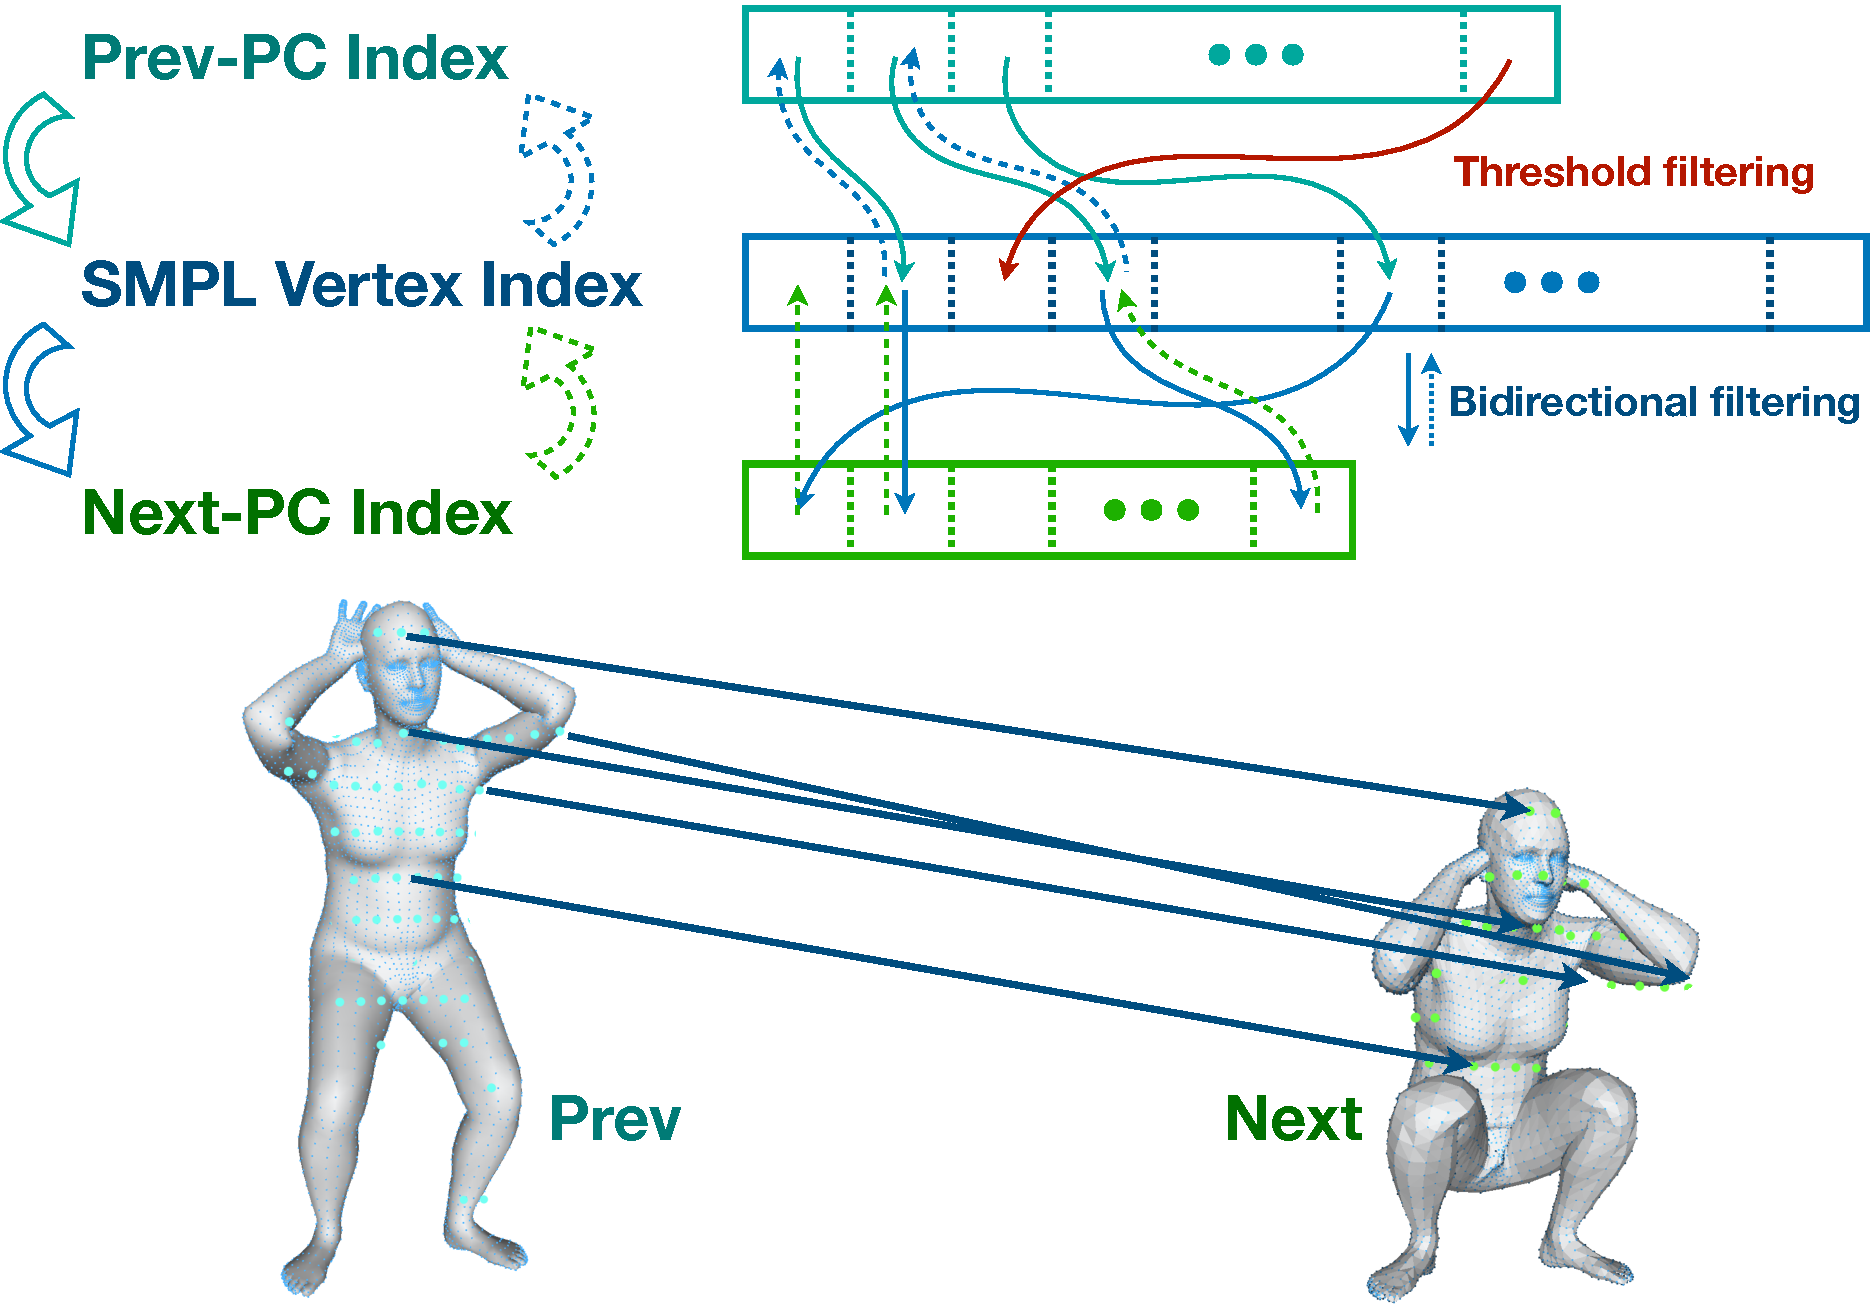
\includegraphics[width=1\columnwidth]{sup_pic/flow.pdf}
    \caption{The pipeline of generating the flow from the previous point cloud to the next point cloud. We associate each synthetic LiDAR point to its nearest SMPL vertex, to establish the correspondence between synthetic LiDAR points across different frames by using SMPL vertices indices as medium, so that we can obtain point-wise motion flow.}
    \label{fig:flow}
    \vspace{-1ex}
\end{figure}
Due to rotation or occlusion, point clouds may flow in and out between consecutive frames, resulting in a lack of temporal correspondence. But for the SMPL~\cite{loper2023smpl} mesh, each mesh vertex can be matched between consecutive frames using vertex index. Therefore, we make a large-scale synthetic dataset, LiDARFlow-Human, by scanning the SMPL mesh surfaces of consecutive frames using a simulated LiDAR to generate simulated LiDAR point clouds (As shown in Figure.~\ref{fig:flow}). Each simulated LiDAR point is matched with its nearest SMPL vertex. Consequently, we use SMPL vertices as a medium to match simulated LiDAR points between frames. By subtracting coordinates, we obtain the point-wise motion flow. Moreover, we set a threshold to filter the distance and build the bidirectional connections to ensure the accuracy of the matching. Specifically, when the nearest distance from vertex to point is smaller than the defined threshold $D$, we think them has the unidirectional connection and we select the unidirectional connection $C_{p2n}$ from previous point cloud to next point clouds, meanwhile we select the unidirectional connection $C_{n2p}$ from next point clouds to previous point clouds. The bidirectional filter are used to delete the unidirectional connection without coincidence, $$Flow_{p2n} = C_{p2n}\cap{C_{n2p}}.$$


% We generate the point-wise motion flow depending on the SMPL vertices. As shown in Figure.~\ref{fig:flow}, the point clouds lack a specific order while the SMPL vertices are ordered temporally. Given that our point clouds possess corresponding SMPL parameters, we generate the SMPL vertices with the full parameters, which completely match with point clouds. Since the SMPL vertices maintain a consistent order, we use these vertices to connect the previous and next point cloud. The connections are established by distance, with each point being paired with its nearest vertex. Moreover, we set a threshold to filter the distance and we build the bidirectional connections to ensure the accuracy of the connections between the previous point cloud and the next point cloud.

% We generate the flow of point clouds depending on the SMPL mesh vertex. As shown in Figure.~\ref{fig:flow}, The point clouds are unordered while the SMPL vertex is ordered, and our point clouds have corresponding SMPL parameters, so we generate the SMPL mesh with the full parameters, which completely matches with point cloud. As the SMPL vertex is in the same order, we use the SMPL vertex to connect the previous and next point cloud. We build the connection by distance, each point has a paired nearest vertex. Moreover, we set a threshold to filter the distance and we build the bidirectional connection to ensure the accuracy of the connection between the previous point cloud and the next point cloud.

\subsection{Dataset and Evaluation Metrics}
We will contribute LiDARFlow-Human, used for training Human Motion Flow Estimator (HMFlow), to the community with corresponding benchmarks. As shown in Table.~\ref{tab:lidarflow_human}, we adopt the evaluation metrics used in ~\cite{puy2020flot,gu2019hplflownet,liu2019flownet3d,wu2019pointpwc}:
\begin{itemize}
\item EPE: End Point Error (meters). $$EPE = \frac{\sum_{i=1}^N \left\| (\vec{(f_{predict})_i}-\vec{(f_{gt})_i}) \right\|_2}{N},$$ where $\vec{(f_{predict})_i}$ and $\vec{(f_{gt})_i}$ are point-wise predicted motion flow and ground truth motion flow, respectively.

\item acc\_strict: percentage of points such that $EPE_i<0.05$ or $EPE_i/ \|\vec{f_i}\|_2<0.05$.
\item acc\_relax: percentage of points such that $EPE_i<0.1$ or $EPE_i/ \|\vec{f_i}\|_2<0.1$.
\item outlier: percentage of points such that $EPE_i>0.3$ or $EPE_i/ \|\vec{f_i}\|_2>0.1$.
\end{itemize}

% The above metrics are computed as follows. The point clouds $\vec{p}, \vec{q}$ are obtained by selecting $n$ random points out of the $N$ provided points in the datasets. The flow is estimated and compared to the ground truth flow $\vec{f}$ on these $n$ selected points. The scores are averaged over the whole validation/test set.
\section{Human Body Segmentation (HBSeg)}

\begin{figure}[t]
    \centering
    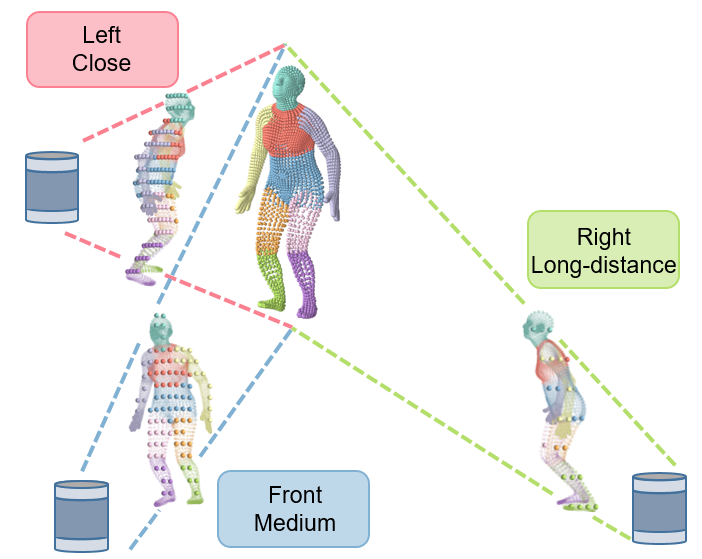
\includegraphics[width=1\columnwidth]{sup_pic/SMPL_1.png}
    \caption{We create a synthetic dataset of 1 million LiDAR human point cloud instances, using the AMASS dataset for 3D human meshes and simulating LiDAR scans from various perspectives and distances for enhancing the diversity of the samples, so as to better simulate the distribution of real-world data. } 
    \label{fig:HBSeg}
    \vspace{-1ex}
\end{figure}

\begin{table}[t]
\caption{Human Motion Flow (HMFlow) Result on LiDARFlow-Human.}
\label{tab:lidarflow_human}
\scalebox{0.95}{
\begin{tabular}{c|c|c|c|c}
\Xhline{1px}
     & EPE$\downarrow$    & acc\_strict$\uparrow$ & acc\_relax$\uparrow$ & outlier$\downarrow$ \\ \hline
FLOT~\cite{puy2020flot} & 0.14 & 83.67             & 95.77           & 0.78  \\ \Xhline{1px}
\end{tabular}
}
\end{table}

\begin{table*}[]\footnotesize
\centering
\caption{Human Body Segmentation (HBSeg) Results on LiDARPart-Human.}
\label{tab:lidarpart_human}
\begin{tabular}{c|c|c|c|c|c|c|c|c|c|c}
\Xhline{1px}
           & head & left-arm & right-arm & up-body & low-body & upleft-leg & upright-leg & lowleft-leg & lowright-leg & mIoU$\uparrow$ \\ \hline
PointNet~\cite{qi2017pointnet}   & 88.2 & 51.2     & 46.6      & 52.1    & 62.6     & 45.8       & 36.2        & 67.4        & 60.2         & 56.7 \\ \hline
PointNet++~\cite{qi2017pointnet++} & 88.6 & 69.5     & 69.9      & 65.4    & 82.2     & 82.7       & 82.5        & 89.1        & 89.4         & 79.9 \\ \hline
PointMLP~\cite{ma2022rethinking}   & 92.0 & 76.1     & 75.2      & 76.7    & 88.0     & 86.3       & 85.8        & 92.8        & 92.3         & 85.0 \\ \hline
PointNeXt~\cite{qian2022pointnext}  & 95.1 & 82.7     & 81.9      & 83.1    & 91.9     & 91.2       & 90.8        & 96.1        & 96.0         & \textbf{89.9} \\ \Xhline{1px}
\end{tabular}
\end{table*}


\begin{table*}[]\scriptsize
\centering
\caption{Supplementary Comparison Experiments on HuCenLife~\cite{xu2023human}. "DM" stands for "Dynamic Method," indicating whether it is a method used for modeling dynamic point cloud videos. For the static methods, which are designed for processing static point clouds, we apply them on each frame of the point cloud sequence and then fuse these frame features after the encoder network by element-wise adding. "SL" stands for "Self-learning", signifying whether the method employs a self-learning mechanism.}
\label{tab:sup_comp_exp}.
\scalebox{0.91}{
\begin{tabular}{l|l|l|c|c|c|c|c|c|c|c|c|c|c|c|c}
\Xhline{1px}
                                                          & DM                                                 & SL                                                 & lift & carry & move & pull\_push & sco-bal & hum-inter & fitness & entertain & sports & bend-over & sit  & walk-stand & mAcc \\ \hline
PointNet~\cite{qi2017pointnet}      & \textcolor{red}{\XSolidBrush} & \textcolor{red}{\XSolidBrush} & 45.5 & 48.8  & 33.3 & 84         & 59.4    & 2.6       & 65.3    & 49.3      & 34.8   & 29.2      & 54.3 & 61         & 47.3 \\ \hline
PointNet++~\cite{qi2017pointnet++}  & \textcolor{red}{\XSolidBrush} & \textcolor{red}{\XSolidBrush} & 49.5 & 45.7  & 35.6 & 52.7       & 59      & 6         & 28.6    & 43.8      & 41.2   & 31.9      & 38.8 & 55         & 40.7 \\ \hline
PointMLP~\cite{ma2022rethinking}    & \textcolor{red}{\XSolidBrush} & \textcolor{red}{\XSolidBrush} & 48.5 & 47.7  & 57.7 & 80.1       & 80.3    & 36.1      & 75.7    & 60.8      & 39.5   & 54.9      & 55.8 & 59.7       & 58.1 \\ \hline
PointNeXt~\cite{qian2022pointnext}  & \textcolor{red}{\XSolidBrush} & \textcolor{red}{\XSolidBrush} & 48.1 & 56.6  & 34.1 & 80         & 85.6    & 22.6      & 50      & 38        & 25.7   & 25.5      & 63.1 & 70.9       & 50   \\ \hline
PCT~\cite{guo2021pct}               & \textcolor{red}{\XSolidBrush} & \textcolor{red}{\XSolidBrush} & 39.7 & 54.9  & 52.3 & 80.2       & 89.8    & 9.8       & 63.3    & 73.6      & 37.7   & 62.5      & 51   & 75.8       & 57.6 \\ \hline
HuCenLife~\cite{xu2023human}        & \textcolor{red}{\XSolidBrush} & \textcolor{red}{\XSolidBrush} & 45   & 44.4  & 52.7 & 81.2       & 86.7    & 23.1      & 81.2    & 54.8      & 41.7   & 54.8      & 53.2 & 70         & 57.4 \\ \hline
PSTNet~\cite{fan2022pstnet}         & \textcolor{green}{\checkmark} & \textcolor{red}{\XSolidBrush} &30.2	&22.6&	61.4&	64.7&	74.6	&21.6&	20.8&	82.4&	39.7	&51.1&	36	&15.4&	43.4 \\ \hline
PSTNet++~\cite{fan2021deep}         & \textcolor{green}{\checkmark} & \textcolor{red}{\XSolidBrush} &31.8&	35.4	&19.4&	77.4&	52.1&	44.8&	65.3&	52.8	&51.6	&43.8&	63&	65.3&	50.2  \\ \hline
P4Transformer~\cite{fan2021point}   & \textcolor{green}{\checkmark} & \textcolor{red}{\XSolidBrush} & 52.6 & 44.1  & 20.6 & 83.8       & 67.5    & 28.1      & 35.4    & 68.7      & 50.6   & 38.8      & 62.6 & 63.8       & 51.4 \\ \hline
PST-Transformer~\cite{fan2022point} & \textcolor{green}{\checkmark} & \textcolor{red}{\XSolidBrush} & 54.2 & 40.3  & 23.4 & 82.6       & 78.5    & 21.8      & 25      & 51.9      & 37.7   & 68.1      & 79   & 74.5       & 53.1 \\ \hline
PPTr~\cite{wen2022point}            & \textcolor{green}{\checkmark} & \textcolor{red}{\XSolidBrush} & 48.2 & 46    & 18   & 79.1       & 71.5    & 20        & 44.7    & 63.7      & 52.4   & 35.6      & 65.4 & 70         & 51.2 \\ \hline
PointMAE~\cite{pang2022masked}      & \textcolor{red}{\XSolidBrush} & \textcolor{green}{\checkmark} & 53.4 & 53.1  & 47.2 & 84.9       & 88.8    & 7.8       & 71.4    & 76.8      & 39.2   & 57.9      & 41.8 & 74.2       & 58   \\ \hline
MaST-Pre~\cite{shen2023masked}      & \textcolor{green}{\checkmark} & \textcolor{green}{\checkmark} & 32.8 & 39.9  & 48.4 & 84.5       & 87.4    & 31.4      & 70.7    & 59.1      & 43.3   & 51.7      & 66.9 & 32.5       & 54.1 \\ \hline
PointCMP~\cite{shen2023pointcmp}    & \textcolor{green}{\checkmark} & \textcolor{green}{\checkmark} & 25.6	&8.3&	56.2	&78.8	&71.9&	7.8&	65.3&	58.6	&52.9&	55.1&	72.9	&19.5&	47.7    \\ \hline
UniPVU-Human                                              & \textcolor{green}{\checkmark} & \textcolor{green}{\checkmark} & 27.1 & 37.3  & 57.1 & 82.6       & 84      & 24.7      & \textbf{85.4}    & 52.1      & \textbf{53.9}   & \textbf{93.8}      & 67.3 & \textbf{76.1}       & \textbf{61.8} \\ \Xhline{1px}
\end{tabular}
}
\end{table*}

% Please add the following required packages to your document preamble:
% \usepackage{multirow}


\subsection{Implementation Details}
To address the absence of 3D human body part segmentation datasets based on LiDAR point clouds, we create a synthetic dataset of 1 million LiDAR human point cloud instances, named LiDARPart-Human, which uses the AMASS dataset for 3D human meshes and simulates LiDAR scans from various perspectives and distances (Figure.~\ref{fig:HBSeg}). These scans incorporate random occlusions and noise to reduce the gap between synthetic and real data. The SMPL mesh vertices, known for their ordered and regular structure, provide 24 human body part labels, but due to the sparsity of LiDAR point clouds, we simplify these to 9 main categories: head, left-arm, right-arm, up-body, low-body, upleft-leg, upright-leg, lowleft-leg, and lowright-leg. Each LiDAR point is automatically labeled with the nearest vertex's body part label. 
\subsection{Dataset and Evaluation Metrics}
Similar to LiDARFlow-Human (Section.~\ref{sec:hmflow}), we also establish a benchmark on LiDARPart-Human and will make it public.
As shown in Table.~\ref{tab:lidarpart_human}, the evaluation metric for LiDARPart-Human is the mean Intersection over Union (mIoU), which is the average of the IoUs calculated for each of the 9 human body parts. 





\section{The Network Design Details for the Tokenizer}
\begin{figure}[t]
    \centering
    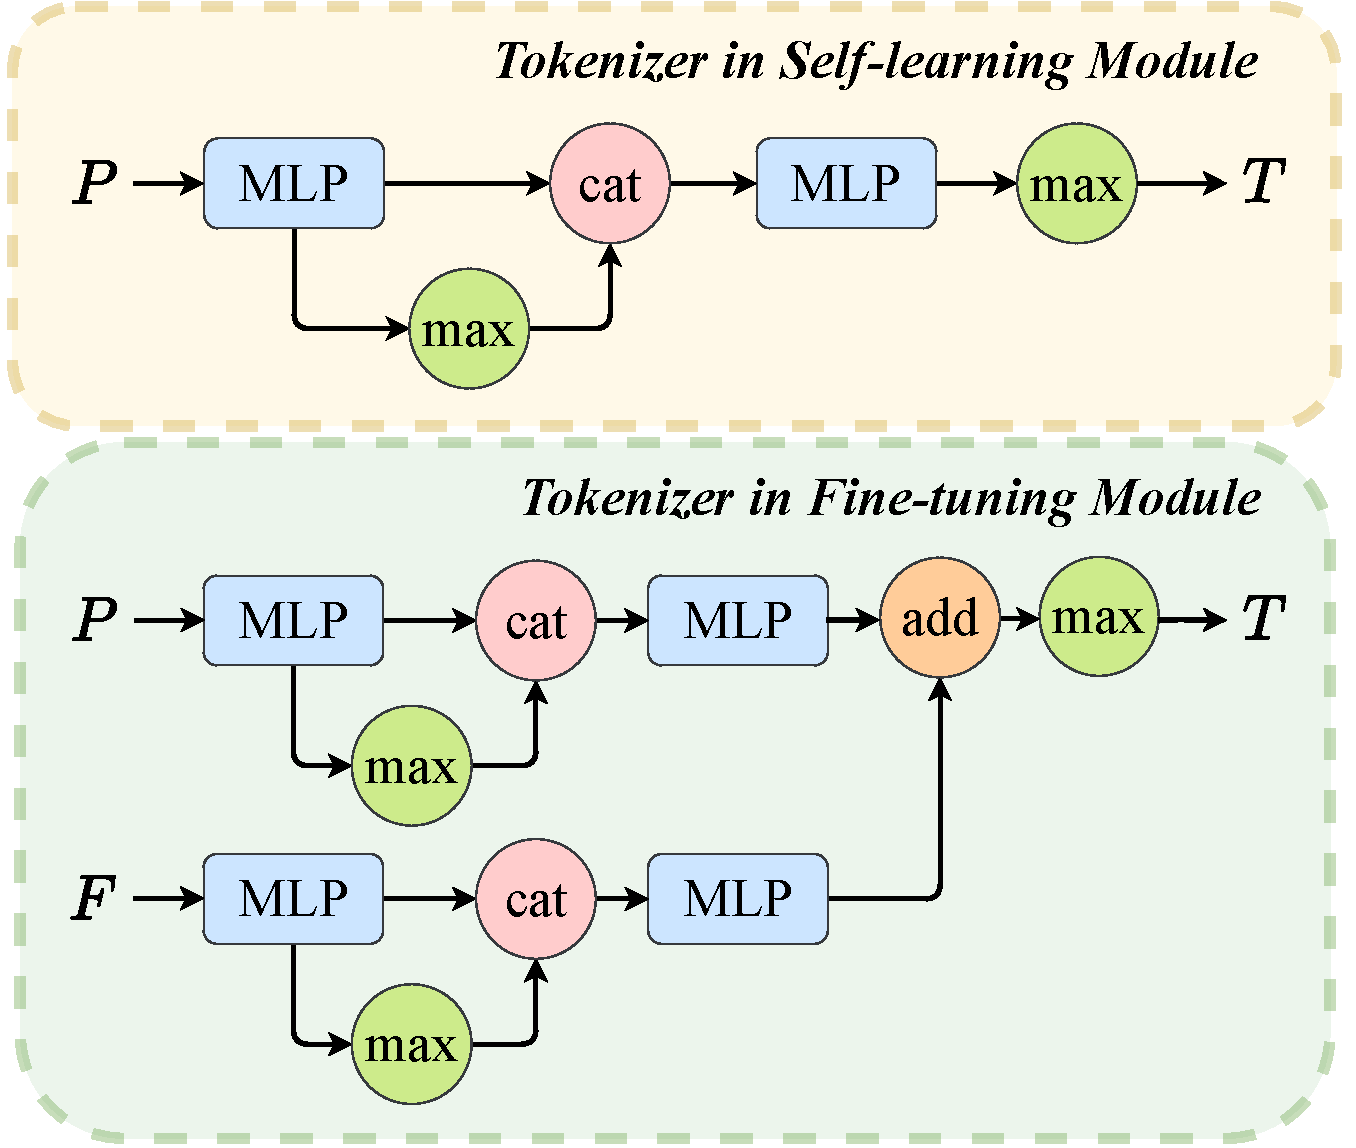
\includegraphics[width=1\columnwidth]{sup_pic/tokenizer_new.drawio.pdf}
    \caption{The network design details for the tokenizer. The primary distinction between the tokenizer in the fine-tuning module and that in the self-learning module lies in the integration of the motion flow features, denoted as $F$. } 
    \label{fig:tokenizer}
    \vspace{-1ex}
\end{figure}
As previously mentioned, in the self-learning module, the motion flow features $F$ are not fused with the part patches features $P$. This design prevents premature leakage of location information of masked tokens to the STEncoder.  
The network design details for the Tokenizer are illustrated in Figure.~\ref{fig:tokenizer}. 
During self-learning, each point of $P$ is mapped to a feature vector using several shared MLPs. Subsequently, max-pooled features are concatenated to each feature vector. These are then processed through several MLPs to expand their dimension to $C=384$. 
During fine-tuning, the same operation is applied to the motion flow $F$. The features of $P$ and $F$ are then fused through element-wise addition. Finally, a max-pooling layer is applied to derive the part token $T$. 


\begin{table}[ht]
\centering
\caption{Comparative Analysis of Model Parameter Numbers in Transformer-Based Dynamic Point Cloud Methods.}
\begin{tabular}{l|cc}
\Xhline{1px}
                                                          & \multicolumn{2}{c}{Num of Params(M)$\downarrow$}            \\ \hline
                                                          & \multicolumn{1}{c|}{Self-learning} & Fine-tuning \\ \hline
P4Transformer~\cite{fan2021point}   & \multicolumn{1}{c|}{/}             & 40.37       \\ \hline
PST-Transformer~\cite{fan2022point} & \multicolumn{1}{c|}{/}             & 60.36       \\ \hline
PPTr~\cite{wen2022point}            & \multicolumn{1}{c|}{/}             & 120.7       \\ \hline
MaST-Pre~\cite{shen2023masked}      & \multicolumn{1}{c|}{140.76}        & 120.66      \\ \hline
UniPVU-Human                                              & \multicolumn{1}{c|}{\textbf{34.92}}         & \textbf{22.48}       \\ \Xhline{1px}
\end{tabular}
\label{tab:model_size}
\end{table}


\section{Supplementary Comparison Experiments on HuCenLife~\cite{xu2023human}}
For more comprehensive and extensive comparisons, we supplement our comparison experiments on HuCenLife~\cite{xu2023human} with methods specifically designed for modeling dynamic point cloud videos~\cite{fan2022pstnet,fan2021point,fan2022point,wen2022point,fan2021deep}. As can be seen from Table.~\ref{tab:sup_comp_exp}, although these methods perform better in categories that require modeling motion features for accurate recognition (Fitness, Sports, Bend-Over, Walk-Stand) than static point cloud methods, there is still a significant performance gap compared to our UniPVU-Human. This confirms the superiority of our method in capturing human motion representations. We also compared our method with self-learning approaches based on contrastive learning~\cite{shen2023pointcmp}. The experimental results demonstrate the superiority of our self-learning mechanism.


\section{Comparative Analysis of Model Parameter Numbers}
Transformer\cite{vaswani2017attention}-based methods~\cite{chen2023pointgpt,liu2023point,zhao2021point,guo2021pct} have achieved considerable performance in point cloud feature extraction. However, their large model size typically results in significant computational demands. As we can see from Table.~\ref{tab:model_size}, the parameter number of other transformer-based dynamic point cloud methods~\cite{fan2021point,fan2022point,wen2022point, shen2023masked}, are several times greater than that of our UniPVU-Human. Our model maintains a parameter number of twenty to thirty million in both the self-learning and fine-tuning stages, which is comparable to ResNet-50~\cite{he2016deep}. Therefore, our UniPVU-Human achieves better performance with fewer parameters, making it a lightweight and effective model well-suited for real-world applications. 


\end{appendix}

% \section{Rationale}
% \label{sec:rationale}
% % 
% Having the supplementary compiled together with the main paper means that:
% % 
% \begin{itemize}
% \item The supplementary can back-reference sections of the main paper, for example, we can refer to \cref{sec:intro};
% \item The main paper can forward reference sub-sections within the supplementary explicitly (e.g. referring to a particular experiment); 
% \item When submitted to arXiv, the supplementary will already included at the end of the paper.
% \end{itemize}
% % 
% To split the supplementary pages from the main paper, you can use \href{https://support.apple.com/en-ca/guide/preview/prvw11793/mac#:~:text=Delete%20a%20page%20from%20a,or%20choose%20Edit%20%3E%20Delete).}{Preview (on macOS)}, \href{https://www.adobe.com/acrobat/how-to/delete-pages-from-pdf.html#:~:text=Choose%20%E2%80%9CTools%E2%80%9D%20%3E%20%E2%80%9COrganize,or%20pages%20from%20the%20file.}{Adobe Acrobat} (on all OSs), as well as \href{https://superuser.com/questions/517986/is-it-possible-to-delete-some-pages-of-a-pdf-document}{command line tools}.
% WARNING: do not forget to delete the supplementary pages from your submission 
% \appendix
% \label{sec:appendix}
% \clearpage
% \clearpage
\setcounter{page}{1}
\begin{appendix}

\section{Overview}
In the supplementary materials, we provide detailed information on the generation of the two datasets used for training HMFlow and HBSeg, along with corresponding benchmarks and evaluation metrics to facilitate their use and assessment in future research. Additionally, we include the implementation details of the Tokenizer in both Self-learning and Fine-tuning stages. For more comprehensive and extensive comparisons, we have expanded our comparison experiments on HuCenLife~\cite{xu2023human} to include methods tailored for modeling dynamic point cloud videos, to demonstrate the superiority of our method in capturing human motion representations. Finally, we also provide additional details regarding the size of the UniPVU-Human model and comparisons with others.
\section{Human Motion Flow (HMFlow)}
\label{sec:hmflow}
\subsection{Implementation Details}
\begin{figure}[ht]
    \centering
    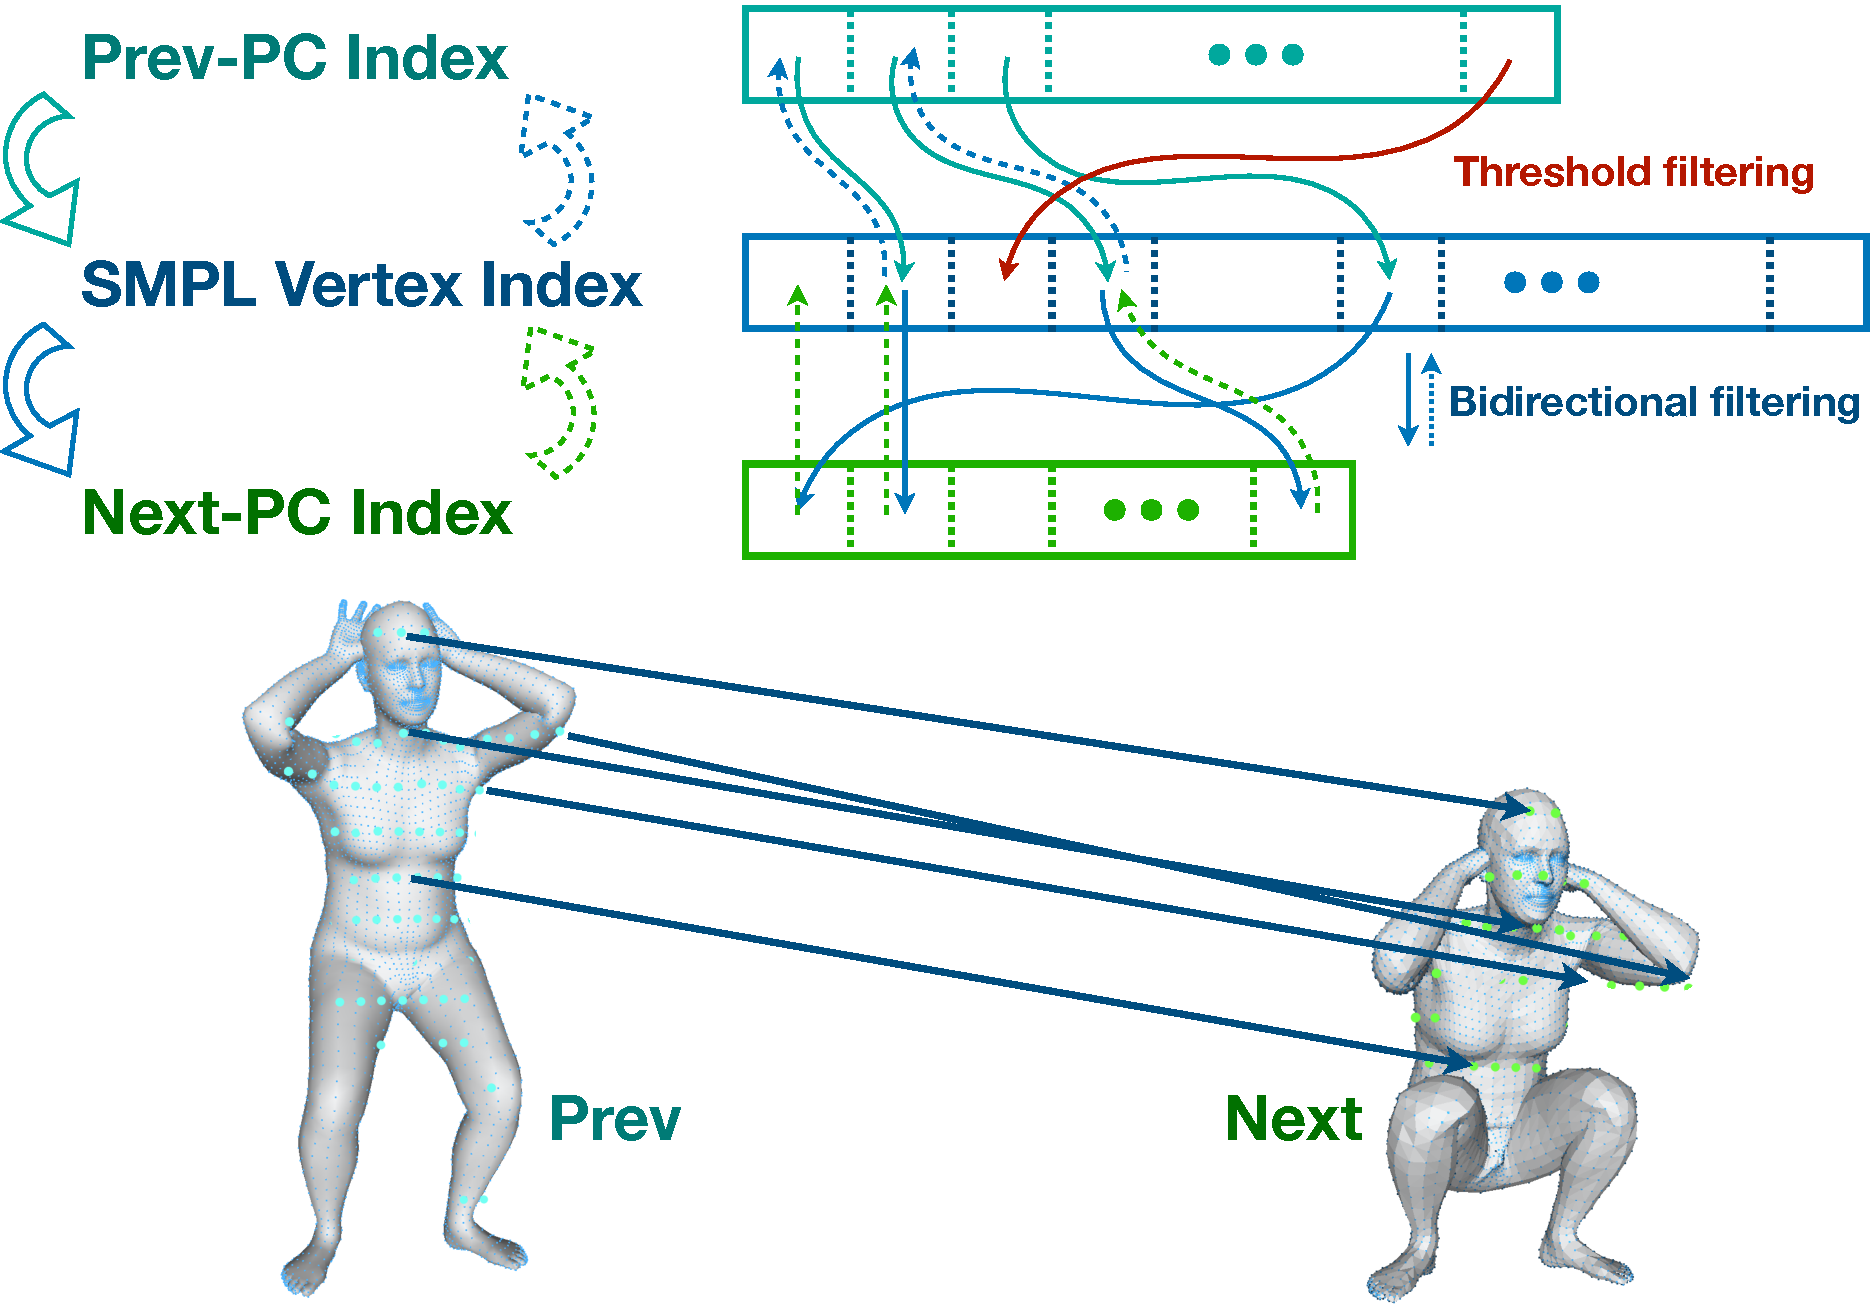
\includegraphics[width=1\columnwidth]{sup_pic/flow.pdf}
    \caption{The pipeline of generating the flow from the previous point cloud to the next point cloud. We associate each synthetic LiDAR point to its nearest SMPL vertex, to establish the correspondence between synthetic LiDAR points across different frames by using SMPL vertices indices as medium, so that we can obtain point-wise motion flow.}
    \label{fig:flow}
    \vspace{-1ex}
\end{figure}
Due to rotation or occlusion, point clouds may flow in and out between consecutive frames, resulting in a lack of temporal correspondence. But for the SMPL~\cite{loper2023smpl} mesh, each mesh vertex can be matched between consecutive frames using vertex index. Therefore, we make a large-scale synthetic dataset, LiDARFlow-Human, by scanning the SMPL mesh surfaces of consecutive frames using a simulated LiDAR to generate simulated LiDAR point clouds (As shown in Figure.~\ref{fig:flow}). Each simulated LiDAR point is matched with its nearest SMPL vertex. Consequently, we use SMPL vertices as a medium to match simulated LiDAR points between frames. By subtracting coordinates, we obtain the point-wise motion flow. Moreover, we set a threshold to filter the distance and build the bidirectional connections to ensure the accuracy of the matching. Specifically, when the nearest distance from vertex to point is smaller than the defined threshold $D$, we think them has the unidirectional connection and we select the unidirectional connection $C_{p2n}$ from previous point cloud to next point clouds, meanwhile we select the unidirectional connection $C_{n2p}$ from next point clouds to previous point clouds. The bidirectional filter are used to delete the unidirectional connection without coincidence, $$Flow_{p2n} = C_{p2n}\cap{C_{n2p}}.$$


% We generate the point-wise motion flow depending on the SMPL vertices. As shown in Figure.~\ref{fig:flow}, the point clouds lack a specific order while the SMPL vertices are ordered temporally. Given that our point clouds possess corresponding SMPL parameters, we generate the SMPL vertices with the full parameters, which completely match with point clouds. Since the SMPL vertices maintain a consistent order, we use these vertices to connect the previous and next point cloud. The connections are established by distance, with each point being paired with its nearest vertex. Moreover, we set a threshold to filter the distance and we build the bidirectional connections to ensure the accuracy of the connections between the previous point cloud and the next point cloud.

% We generate the flow of point clouds depending on the SMPL mesh vertex. As shown in Figure.~\ref{fig:flow}, The point clouds are unordered while the SMPL vertex is ordered, and our point clouds have corresponding SMPL parameters, so we generate the SMPL mesh with the full parameters, which completely matches with point cloud. As the SMPL vertex is in the same order, we use the SMPL vertex to connect the previous and next point cloud. We build the connection by distance, each point has a paired nearest vertex. Moreover, we set a threshold to filter the distance and we build the bidirectional connection to ensure the accuracy of the connection between the previous point cloud and the next point cloud.

\subsection{Dataset and Evaluation Metrics}
We will contribute LiDARFlow-Human, used for training Human Motion Flow Estimator (HMFlow), to the community with corresponding benchmarks. As shown in Table.~\ref{tab:lidarflow_human}, we adopt the evaluation metrics used in ~\cite{puy2020flot,gu2019hplflownet,liu2019flownet3d,wu2019pointpwc}:
\begin{itemize}
\item EPE: End Point Error (meters). $$EPE = \frac{\sum_{i=1}^N \left\| (\vec{(f_{predict})_i}-\vec{(f_{gt})_i}) \right\|_2}{N},$$ where $\vec{(f_{predict})_i}$ and $\vec{(f_{gt})_i}$ are point-wise predicted motion flow and ground truth motion flow, respectively.

\item acc\_strict: percentage of points such that $EPE_i<0.05$ or $EPE_i/ \|\vec{f_i}\|_2<0.05$.
\item acc\_relax: percentage of points such that $EPE_i<0.1$ or $EPE_i/ \|\vec{f_i}\|_2<0.1$.
\item outlier: percentage of points such that $EPE_i>0.3$ or $EPE_i/ \|\vec{f_i}\|_2>0.1$.
\end{itemize}

% The above metrics are computed as follows. The point clouds $\vec{p}, \vec{q}$ are obtained by selecting $n$ random points out of the $N$ provided points in the datasets. The flow is estimated and compared to the ground truth flow $\vec{f}$ on these $n$ selected points. The scores are averaged over the whole validation/test set.
\section{Human Body Segmentation (HBSeg)}

\begin{figure}[t]
    \centering
    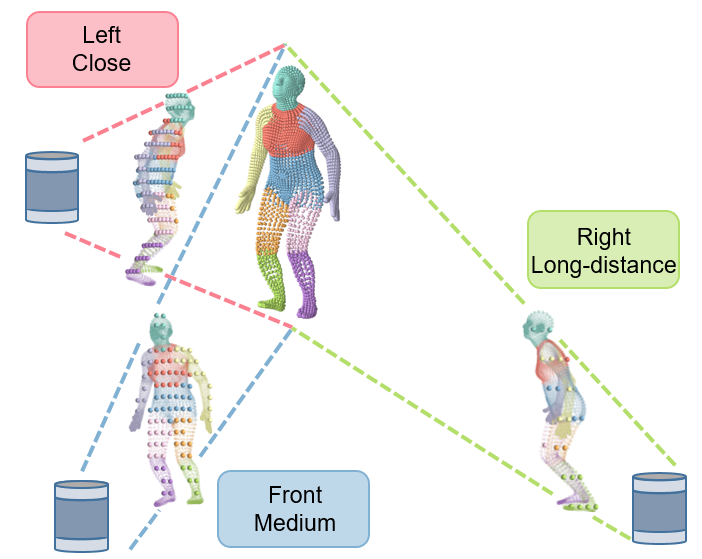
\includegraphics[width=1\columnwidth]{sup_pic/SMPL_1.png}
    \caption{We create a synthetic dataset of 1 million LiDAR human point cloud instances, using the AMASS dataset for 3D human meshes and simulating LiDAR scans from various perspectives and distances for enhancing the diversity of the samples, so as to better simulate the distribution of real-world data. } 
    \label{fig:HBSeg}
    \vspace{-1ex}
\end{figure}

\begin{table}[t]
\caption{Human Motion Flow (HMFlow) Result on LiDARFlow-Human.}
\label{tab:lidarflow_human}
\scalebox{0.95}{
\begin{tabular}{c|c|c|c|c}
\Xhline{1px}
     & EPE$\downarrow$    & acc\_strict$\uparrow$ & acc\_relax$\uparrow$ & outlier$\downarrow$ \\ \hline
FLOT~\cite{puy2020flot} & 0.14 & 83.67             & 95.77           & 0.78  \\ \Xhline{1px}
\end{tabular}
}
\end{table}

\begin{table*}[]\footnotesize
\centering
\caption{Human Body Segmentation (HBSeg) Results on LiDARPart-Human.}
\label{tab:lidarpart_human}
\begin{tabular}{c|c|c|c|c|c|c|c|c|c|c}
\Xhline{1px}
           & head & left-arm & right-arm & up-body & low-body & upleft-leg & upright-leg & lowleft-leg & lowright-leg & mIoU$\uparrow$ \\ \hline
PointNet~\cite{qi2017pointnet}   & 88.2 & 51.2     & 46.6      & 52.1    & 62.6     & 45.8       & 36.2        & 67.4        & 60.2         & 56.7 \\ \hline
PointNet++~\cite{qi2017pointnet++} & 88.6 & 69.5     & 69.9      & 65.4    & 82.2     & 82.7       & 82.5        & 89.1        & 89.4         & 79.9 \\ \hline
PointMLP~\cite{ma2022rethinking}   & 92.0 & 76.1     & 75.2      & 76.7    & 88.0     & 86.3       & 85.8        & 92.8        & 92.3         & 85.0 \\ \hline
PointNeXt~\cite{qian2022pointnext}  & 95.1 & 82.7     & 81.9      & 83.1    & 91.9     & 91.2       & 90.8        & 96.1        & 96.0         & \textbf{89.9} \\ \Xhline{1px}
\end{tabular}
\end{table*}


\begin{table*}[]\scriptsize
\centering
\caption{Supplementary Comparison Experiments on HuCenLife~\cite{xu2023human}. "DM" stands for "Dynamic Method," indicating whether it is a method used for modeling dynamic point cloud videos. For the static methods, which are designed for processing static point clouds, we apply them on each frame of the point cloud sequence and then fuse these frame features after the encoder network by element-wise adding. "SL" stands for "Self-learning", signifying whether the method employs a self-learning mechanism.}
\label{tab:sup_comp_exp}.
\scalebox{0.91}{
\begin{tabular}{l|l|l|c|c|c|c|c|c|c|c|c|c|c|c|c}
\Xhline{1px}
                                                          & DM                                                 & SL                                                 & lift & carry & move & pull\_push & sco-bal & hum-inter & fitness & entertain & sports & bend-over & sit  & walk-stand & mAcc \\ \hline
PointNet~\cite{qi2017pointnet}      & \textcolor{red}{\XSolidBrush} & \textcolor{red}{\XSolidBrush} & 45.5 & 48.8  & 33.3 & 84         & 59.4    & 2.6       & 65.3    & 49.3      & 34.8   & 29.2      & 54.3 & 61         & 47.3 \\ \hline
PointNet++~\cite{qi2017pointnet++}  & \textcolor{red}{\XSolidBrush} & \textcolor{red}{\XSolidBrush} & 49.5 & 45.7  & 35.6 & 52.7       & 59      & 6         & 28.6    & 43.8      & 41.2   & 31.9      & 38.8 & 55         & 40.7 \\ \hline
PointMLP~\cite{ma2022rethinking}    & \textcolor{red}{\XSolidBrush} & \textcolor{red}{\XSolidBrush} & 48.5 & 47.7  & 57.7 & 80.1       & 80.3    & 36.1      & 75.7    & 60.8      & 39.5   & 54.9      & 55.8 & 59.7       & 58.1 \\ \hline
PointNeXt~\cite{qian2022pointnext}  & \textcolor{red}{\XSolidBrush} & \textcolor{red}{\XSolidBrush} & 48.1 & 56.6  & 34.1 & 80         & 85.6    & 22.6      & 50      & 38        & 25.7   & 25.5      & 63.1 & 70.9       & 50   \\ \hline
PCT~\cite{guo2021pct}               & \textcolor{red}{\XSolidBrush} & \textcolor{red}{\XSolidBrush} & 39.7 & 54.9  & 52.3 & 80.2       & 89.8    & 9.8       & 63.3    & 73.6      & 37.7   & 62.5      & 51   & 75.8       & 57.6 \\ \hline
HuCenLife~\cite{xu2023human}        & \textcolor{red}{\XSolidBrush} & \textcolor{red}{\XSolidBrush} & 45   & 44.4  & 52.7 & 81.2       & 86.7    & 23.1      & 81.2    & 54.8      & 41.7   & 54.8      & 53.2 & 70         & 57.4 \\ \hline
PSTNet~\cite{fan2022pstnet}         & \textcolor{green}{\checkmark} & \textcolor{red}{\XSolidBrush} &30.2	&22.6&	61.4&	64.7&	74.6	&21.6&	20.8&	82.4&	39.7	&51.1&	36	&15.4&	43.4 \\ \hline
PSTNet++~\cite{fan2021deep}         & \textcolor{green}{\checkmark} & \textcolor{red}{\XSolidBrush} &31.8&	35.4	&19.4&	77.4&	52.1&	44.8&	65.3&	52.8	&51.6	&43.8&	63&	65.3&	50.2  \\ \hline
P4Transformer~\cite{fan2021point}   & \textcolor{green}{\checkmark} & \textcolor{red}{\XSolidBrush} & 52.6 & 44.1  & 20.6 & 83.8       & 67.5    & 28.1      & 35.4    & 68.7      & 50.6   & 38.8      & 62.6 & 63.8       & 51.4 \\ \hline
PST-Transformer~\cite{fan2022point} & \textcolor{green}{\checkmark} & \textcolor{red}{\XSolidBrush} & 54.2 & 40.3  & 23.4 & 82.6       & 78.5    & 21.8      & 25      & 51.9      & 37.7   & 68.1      & 79   & 74.5       & 53.1 \\ \hline
PPTr~\cite{wen2022point}            & \textcolor{green}{\checkmark} & \textcolor{red}{\XSolidBrush} & 48.2 & 46    & 18   & 79.1       & 71.5    & 20        & 44.7    & 63.7      & 52.4   & 35.6      & 65.4 & 70         & 51.2 \\ \hline
PointMAE~\cite{pang2022masked}      & \textcolor{red}{\XSolidBrush} & \textcolor{green}{\checkmark} & 53.4 & 53.1  & 47.2 & 84.9       & 88.8    & 7.8       & 71.4    & 76.8      & 39.2   & 57.9      & 41.8 & 74.2       & 58   \\ \hline
MaST-Pre~\cite{shen2023masked}      & \textcolor{green}{\checkmark} & \textcolor{green}{\checkmark} & 32.8 & 39.9  & 48.4 & 84.5       & 87.4    & 31.4      & 70.7    & 59.1      & 43.3   & 51.7      & 66.9 & 32.5       & 54.1 \\ \hline
PointCMP~\cite{shen2023pointcmp}    & \textcolor{green}{\checkmark} & \textcolor{green}{\checkmark} & 25.6	&8.3&	56.2	&78.8	&71.9&	7.8&	65.3&	58.6	&52.9&	55.1&	72.9	&19.5&	47.7    \\ \hline
UniPVU-Human                                              & \textcolor{green}{\checkmark} & \textcolor{green}{\checkmark} & 27.1 & 37.3  & 57.1 & 82.6       & 84      & 24.7      & \textbf{85.4}    & 52.1      & \textbf{53.9}   & \textbf{93.8}      & 67.3 & \textbf{76.1}       & \textbf{61.8} \\ \Xhline{1px}
\end{tabular}
}
\end{table*}

% Please add the following required packages to your document preamble:
% \usepackage{multirow}


\subsection{Implementation Details}
To address the absence of 3D human body part segmentation datasets based on LiDAR point clouds, we create a synthetic dataset of 1 million LiDAR human point cloud instances, named LiDARPart-Human, which uses the AMASS dataset for 3D human meshes and simulates LiDAR scans from various perspectives and distances (Figure.~\ref{fig:HBSeg}). These scans incorporate random occlusions and noise to reduce the gap between synthetic and real data. The SMPL mesh vertices, known for their ordered and regular structure, provide 24 human body part labels, but due to the sparsity of LiDAR point clouds, we simplify these to 9 main categories: head, left-arm, right-arm, up-body, low-body, upleft-leg, upright-leg, lowleft-leg, and lowright-leg. Each LiDAR point is automatically labeled with the nearest vertex's body part label. 
\subsection{Dataset and Evaluation Metrics}
Similar to LiDARFlow-Human (Section.~\ref{sec:hmflow}), we also establish a benchmark on LiDARPart-Human and will make it public.
As shown in Table.~\ref{tab:lidarpart_human}, the evaluation metric for LiDARPart-Human is the mean Intersection over Union (mIoU), which is the average of the IoUs calculated for each of the 9 human body parts. 





\section{The Network Design Details for the Tokenizer}
\begin{figure}[t]
    \centering
    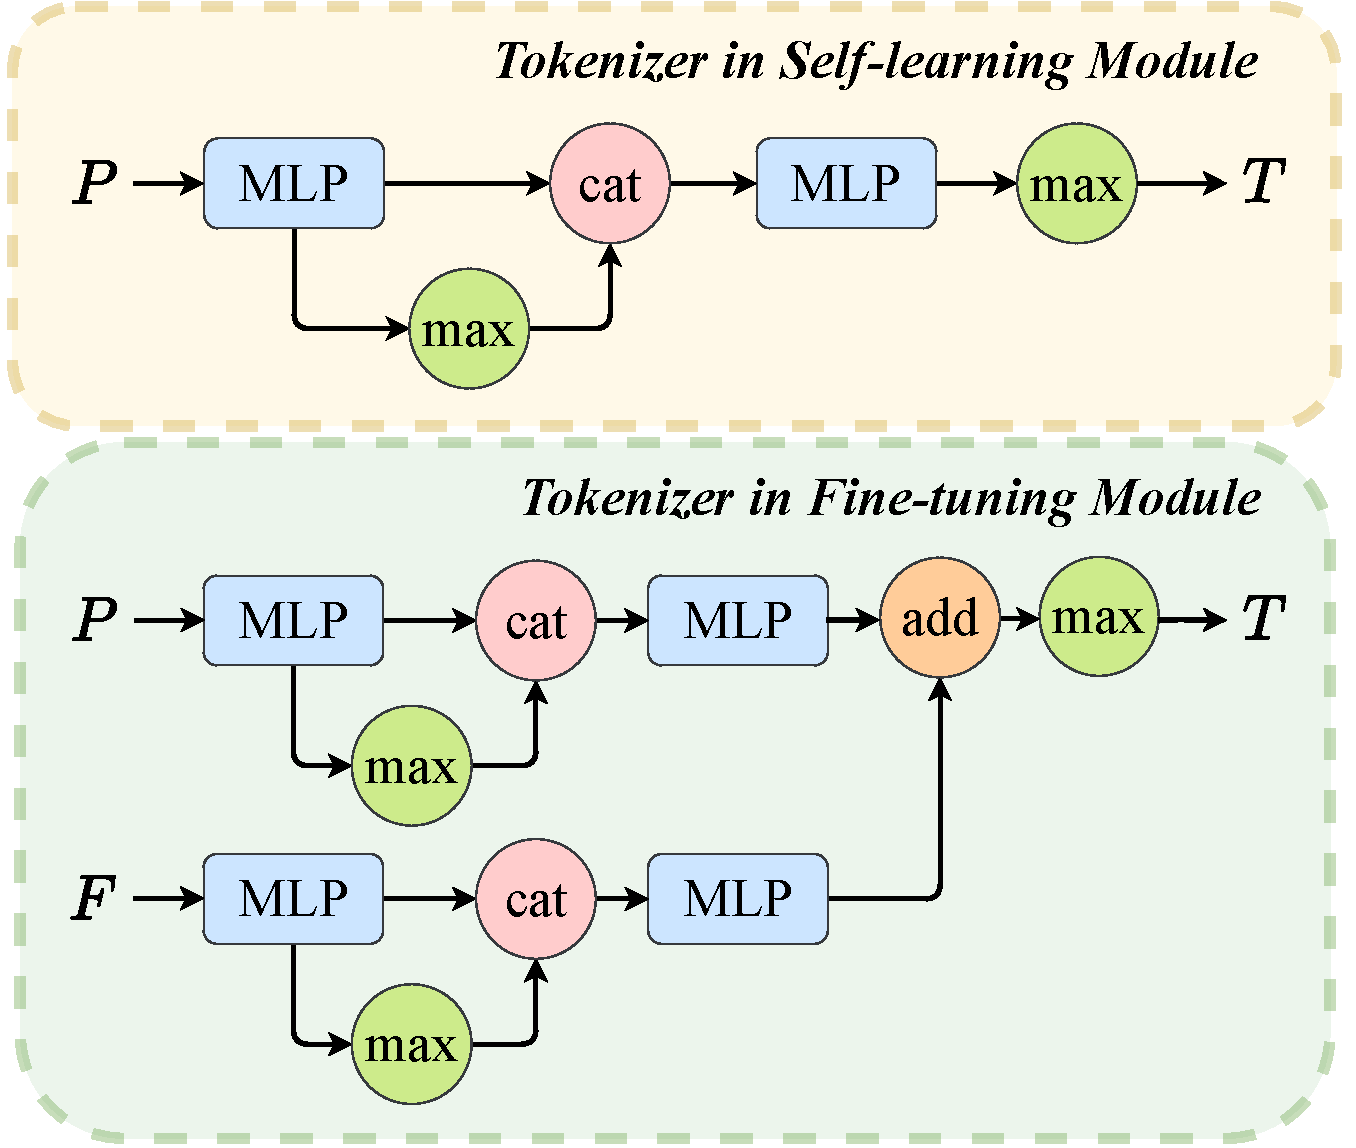
\includegraphics[width=1\columnwidth]{sup_pic/tokenizer_new.drawio.pdf}
    \caption{The network design details for the tokenizer. The primary distinction between the tokenizer in the fine-tuning module and that in the self-learning module lies in the integration of the motion flow features, denoted as $F$. } 
    \label{fig:tokenizer}
    \vspace{-1ex}
\end{figure}
As previously mentioned, in the self-learning module, the motion flow features $F$ are not fused with the part patches features $P$. This design prevents premature leakage of location information of masked tokens to the STEncoder.  
The network design details for the Tokenizer are illustrated in Figure.~\ref{fig:tokenizer}. 
During self-learning, each point of $P$ is mapped to a feature vector using several shared MLPs. Subsequently, max-pooled features are concatenated to each feature vector. These are then processed through several MLPs to expand their dimension to $C=384$. 
During fine-tuning, the same operation is applied to the motion flow $F$. The features of $P$ and $F$ are then fused through element-wise addition. Finally, a max-pooling layer is applied to derive the part token $T$. 


\begin{table}[ht]
\centering
\caption{Comparative Analysis of Model Parameter Numbers in Transformer-Based Dynamic Point Cloud Methods.}
\begin{tabular}{l|cc}
\Xhline{1px}
                                                          & \multicolumn{2}{c}{Num of Params(M)$\downarrow$}            \\ \hline
                                                          & \multicolumn{1}{c|}{Self-learning} & Fine-tuning \\ \hline
P4Transformer~\cite{fan2021point}   & \multicolumn{1}{c|}{/}             & 40.37       \\ \hline
PST-Transformer~\cite{fan2022point} & \multicolumn{1}{c|}{/}             & 60.36       \\ \hline
PPTr~\cite{wen2022point}            & \multicolumn{1}{c|}{/}             & 120.7       \\ \hline
MaST-Pre~\cite{shen2023masked}      & \multicolumn{1}{c|}{140.76}        & 120.66      \\ \hline
UniPVU-Human                                              & \multicolumn{1}{c|}{\textbf{34.92}}         & \textbf{22.48}       \\ \Xhline{1px}
\end{tabular}
\label{tab:model_size}
\end{table}


\section{Supplementary Comparison Experiments on HuCenLife~\cite{xu2023human}}
For more comprehensive and extensive comparisons, we supplement our comparison experiments on HuCenLife~\cite{xu2023human} with methods specifically designed for modeling dynamic point cloud videos~\cite{fan2022pstnet,fan2021point,fan2022point,wen2022point,fan2021deep}. As can be seen from Table.~\ref{tab:sup_comp_exp}, although these methods perform better in categories that require modeling motion features for accurate recognition (Fitness, Sports, Bend-Over, Walk-Stand) than static point cloud methods, there is still a significant performance gap compared to our UniPVU-Human. This confirms the superiority of our method in capturing human motion representations. We also compared our method with self-learning approaches based on contrastive learning~\cite{shen2023pointcmp}. The experimental results demonstrate the superiority of our self-learning mechanism.


\section{Comparative Analysis of Model Parameter Numbers}
Transformer\cite{vaswani2017attention}-based methods~\cite{chen2023pointgpt,liu2023point,zhao2021point,guo2021pct} have achieved considerable performance in point cloud feature extraction. However, their large model size typically results in significant computational demands. As we can see from Table.~\ref{tab:model_size}, the parameter number of other transformer-based dynamic point cloud methods~\cite{fan2021point,fan2022point,wen2022point, shen2023masked}, are several times greater than that of our UniPVU-Human. Our model maintains a parameter number of twenty to thirty million in both the self-learning and fine-tuning stages, which is comparable to ResNet-50~\cite{he2016deep}. Therefore, our UniPVU-Human achieves better performance with fewer parameters, making it a lightweight and effective model well-suited for real-world applications. 


\end{appendix}

% \section{Rationale}
% \label{sec:rationale}
% % 
% Having the supplementary compiled together with the main paper means that:
% % 
% \begin{itemize}
% \item The supplementary can back-reference sections of the main paper, for example, we can refer to \cref{sec:intro};
% \item The main paper can forward reference sub-sections within the supplementary explicitly (e.g. referring to a particular experiment); 
% \item When submitted to arXiv, the supplementary will already included at the end of the paper.
% \end{itemize}
% % 
% To split the supplementary pages from the main paper, you can use \href{https://support.apple.com/en-ca/guide/preview/prvw11793/mac#:~:text=Delete%20a%20page%20from%20a,or%20choose%20Edit%20%3E%20Delete).}{Preview (on macOS)}, \href{https://www.adobe.com/acrobat/how-to/delete-pages-from-pdf.html#:~:text=Choose%20%E2%80%9CTools%E2%80%9D%20%3E%20%E2%80%9COrganize,or%20pages%20from%20the%20file.}{Adobe Acrobat} (on all OSs), as well as \href{https://superuser.com/questions/517986/is-it-possible-to-delete-some-pages-of-a-pdf-document}{command line tools}.

\end{document}
